\documentclass[letterpaper,11pt]{article}

\usepackage[margin=1in]{geometry}
\usepackage[tight,nice]{units}
\usepackage{graphicx,color,float,url,amsmath,parskip,multicol}
%\usepackage[super]{cite}
\usepackage{subfigure}
\usepackage{listings}
\usepackage{sectsty}
\usepackage{appendix}
\usepackage{amssymb}
\usepackage{url}
\sectionfont{\normalsize}
\subsectionfont{\normalsize}
\title{\normalsize}
\usepackage{setspace}
\usepackage{natbib}
\usepackage[nottoc,numbib]{tocbibind}
\usepackage{fancyhdr}
\usepackage[outercaption]{sidecap}
\usepackage{eqnarray}
\usepackage{mathrsfs, amsmath, amsfonts, xspace}
\usepackage[pagewise, mathlines]{lineno}

\usepackage{hyperref}
\hypersetup{colorlinks=true,linkcolor=blue,citecolor=blue}

%% =============================================================================
%% My eqs
%% =============================================================================
\renewcommand{\bibname}{REFERENCES}
\newcommand{\SimPEG}{\textsc{SimPEG}\xspace}
\renewcommand{\div}{\nabla\cdot}
\newcommand{\grad}{\vec \nabla}
\newcommand{\curl}{{\vec \nabla}\times}
\newcommand {\J}{{\vec J}}
\renewcommand{\H}{{\vec H}}
\newcommand {\E}{{\vec E}}
\newcommand{\siginf}{\sigma_\infty}
\newcommand{\dsig}{\triangle\sigma}
\newcommand{\dcurl}{{\mathbf C}}
\newcommand{\dgrad}{{\mathbf G}}
\newcommand{\Acf}{{\mathbf A_c^f}}
\newcommand{\Ace}{{\mathbf A_c^e}}
\renewcommand{\S}{{\mathbf \Sigma}}
\newcommand{\St}{{\mathbf \Sigma_\tau}}
\newcommand{\T}{{\mathbf T}}
\newcommand{\Tt}{{\mathbf T_\tau}}
\newcommand{\diag}{\mathbf{diag}}
\newcommand{\M}{{\mathbf M}}
\newcommand{\MfMui}{{\M^f_{\mu^{-1}}}}
\newcommand{\MfMuoi}{{\M^f_{\mu_0^{-1}}}}
\newcommand{\dMfMuI}{{d_m (\M^f_{\mu^{-1}})^{-1}}}
\newcommand{\dMfMuoI}{{d_m (\M^f_{\mu_0^{-1}})^{-1}}}
\newcommand{\MeSig}{{\M^e_\sigma}}
\newcommand{\MeSigInf}{{\M^e_{\sigma_\infty}}}
\newcommand{\MeSigInfEtab}{{\M^e_{\sigma_\infty \bar{\eta}}}}
\newcommand{\MeSigInfEtat}{{\M^e_{\sigma_\infty \peta}}}
\newcommand{\MedSig}{{\M^e_{\triangle\sigma}}}
\newcommand{\MeSigO}{{\M^e_{\sigma_0}}}
\newcommand{\Me}{{\M^e}}
\newcommand{\Js}{\mathbf{J}^s}
\newcommand{\Mes}[1]{{\M^e_{#1}}}
\newcommand{\Mee}{{\M^e_e}}
\newcommand{\Mej}{{\M^e_j}}
\newcommand{\BigO}[1]{\mathcal{O}\bigl(#1\bigr)}
\newcommand{\bE}{\mathbf{E}}
\newcommand{\bEp}{\mathbf{E}^p}
\newcommand{\bB}{\mathbf{B}}
\newcommand{\bBp}{\mathbf{B}^p}
\newcommand{\bEs}{\mathbf{E}^s}
\newcommand{\bBs}{\mathbf{B}^s}
\newcommand{\bH}{\mathbf{H}}
\newcommand{\B}{\vec{B}}
\newcommand{\D}{\vec{D}}
\renewcommand{\H}{\vec{H}}
\newcommand{\s}{\vec{s}}
\newcommand{\bfJ}{\bf{J}}
\newcommand{\vecm}{\vec m}
\renewcommand{\Re}{\mathsf{Re}}
\renewcommand{\Im}{\mathsf{Im}}
\renewcommand {\j}  { {\vec j} }
\newcommand {\h}  { {\vec h} }
\renewcommand {\b}  { {\vec b} }
\newcommand {\e}  { {\vec e} }
\renewcommand {\d}  { {\vec d} }
\renewcommand {\u}  { {\vec u} }

\renewcommand {\dj}  { {\mathbf{j} } }
\renewcommand {\dh}  { {\mathbf{h} } }
\newcommand {\db}  { {\mathbf{b} } }
\newcommand {\de}  { {\mathbf{e} } }

\newcommand{\vol}{\mathbf{v}}
\newcommand{\I}{\vec{I}}
\newcommand{\A}{\mathbf{A}}
\newcommand{\bI}{\mathbf{I}}
\newcommand{\bus}{\mathbf{u}^s}
\newcommand{\brhss}{\mathbf{rhs}_s}
\newcommand{\bup}{\mathbf{u}^p}
\newcommand{\brhs}{\mathbf{rhs}}
%%-------------------------------
\newcommand{\bon}{b^{on}(t)}
\newcommand{\bp}{b^{p}}
\newcommand{\dbondt}{\frac{db^{on}(t)}{dt}}
\newcommand{\dfdt}{\frac{df(t)}{dt}}
\newcommand{\dfdtdsiginf}{\frac{\partial\frac{df(t)}{dt}}{\partial\siginf}}
\newcommand{\dfdsiginf}{\frac{\partial f(t)}{\partial\siginf}}
\newcommand{\dbgdsiginf}{\frac{\partial b^{Impulse}(t)}{\partial\siginf}}
\newcommand{\digint}{\frac{2}{\pi}\int_0^{\infty}}
\newcommand{\Gbiot}{\mathbf{G}_{Biot}}
%%-------------------------------
\newcommand{\peta}{\tilde{\eta}}
\newcommand{\petadt}{\frac{\partial \tilde{\eta}}{\partial t}}
\newcommand{\eFmax}{\e^{\ F}_{max}}
\newcommand{\eref}{\e^{\ ref}}
\newcommand{\jref}{\j^{\ ref}}
\newcommand{\dip}{d^{IP}}
\newcommand{\sigpert}{\delta\sigma}
\newcommand{\bzip}{b_z^{IP}}
\newcommand{\dbzdtip}{\frac{\partial b_z^{IP}}{\partial t}}
\newcommand{\dbdt}{\frac{\partial \b}{\partial t}}


%% =============================================================================
%% End of my eqs
%% =============================================================================
\pagestyle{fancy}

\fancyhead{}
\fancyhead[L]{Thesis Proposal}
\fancyhead[R]{Seogi Kang}

\begin{document}
\begin{titlepage}
 
\begin{center}
\textsc{Ph.D. Thesis Proposal}
\end{center}

\vspace{1cm}
 
\large
\begin{center}
\line(1,0){450}
\vspace{0.25cm}
\textbf{\LARGE On recovering distributed IP information from time domain EM data}
\line(1,0){450}
\end{center}

\normalsize

\vspace{1cm}

\begin{center}
\textsc{\large Seogi Kang}
\end{center}

\begin{center}
\begin{footnotesize}
November 27, 2015
\end{footnotesize}
\end{center}

\vspace{2cm}

\begin{center}
\begin{tabular}{l r}
\textit{Supervisor:} \hspace{8cm} & \textit{External Examiner:} \\
\textsc{Douglas W. Oldenburg} & \textsc{Christian Schoof} \\
 & \\
 & \\
\textit{Committee Members:} & \textit{Examination Chair:}\\
\textsc{Eldad Haber} & \textsc{?}\\
\textsc{Randy Enkin} & \\
\end{tabular}
\end{center}

\vspace{2cm}

\begin{center}
\textsc{Department of Earth, Ocean, and Atmospheric Sciences}\\
\textsc{University of British Columbia}\\
\end{center}

\end{titlepage}
\newpage

\tableofcontents
\newpage

\section{INTRODUCTION}
The electrical conductivity of earth materials can be frequency dependent with the effective conductivity decreasing with decreasing frequency due to the buildup of electric charges that occur under the application of an electric field. Effectively, the rock is electrically polarized. 
Applications of induced polarization (IP) surveys to find chargeable material  have been particularly successful in mineral exploration for disseminated sulphide or porphyry deposits \cite[]{Pelton1978, Fink1990} and also in geotechnical and environmental problems \cite[]{Kemna2012}. 

Polarization charges can accumulate whenever there is an electric field in a medium. In controlled source surveys, the transmitter can be a galvanic source (a generator attached to two grounded electrodes), or an inductive source (arising from currents flowing in a wire loop). Most research and application has focused upon using grounded electrodes and measuring electric fields; this is called an EIP survey \cite[]{seigel1959}. Magnetic fields arising from polarization currents (MIP survey) have also been successfully used, particularly in mineral exploration geologies characterized by a conductive overburden \cite[]{seigel1974}. 

In recent years attention has also turned towards the use of inductive sources. Inductive source IP (ISIP), can have transmitters in the air or on the ground and the waveforms can be in either the frequency or time domain. Recently  \cite[]{Marchant2012b} showed how, by collecting data at two frequencies, it was possible to measure data that depended purely on IP signals and that these data can be inverted to recover a 3D distribution of chargeability. 
For time domain systems the observations of negative transients in coincident loop systems provide an distinctive verification of the existence of chargeable material \cite[]{Weidelt1982}. These negative transients have been frequently observed \cite[]{SmithandKlein,Kang2015a}. The effects of chargeable objects on time domain system with inductive sources have been carefully investigated \cite[]{Smith1988a,Flis1989,ElKaliouby2004, Marchant2014} and approximate interpretation tools \cite[]{Kratzer2012,Hodges2014,Kwan2015} are being developed. The ability to fully invert these data in 3D is still lacking. 

Extracting information about the complex conductivity can be done in a variety of ways. In principle it can be solved by finding a function $\sigma(x,y,z,\omega)$ or parameterizing the complex conductivity, usually with a Cole-Cole type model, and finding the distribution of those parameters \cite[]{Fiandaca2012, Marchant2013,Xu2013}. Traditionally, however, with EIP and time domain waveforms, one first estimates the background conductivity from the asymptotic on-time data and then inverts off-time data to recover information about ``chargeability'' \cite[]{doug1994}. This is carried out by solving an inverse problem using a linear function where the sensitivities depend upon geometry of the survey and the background conductivity. The recovered values are really pseudo-chargeability, and they have the same units as the data (eg. msec, mV/V). The same procedure can be used in frequency domain experiments but the data might have units of mrad and pfe (percent frequency effect). Inversion of IP data to recover 2D or 3D distributions of pseudo-chargeability are now commonly carried out \cite[]{Kemna2012}. These inversions delineate locations of high pseudo-chargeability and the geometry of the bodies. MIP data can be inverted with the same methodology \cite[]{Chen2003}. 

The physical mechanisms by which polarization charges and currents are established in the ground are independent of the type of transmitter and waveform; the important quantity is the time history of the electric field within the earth. The challenge posed by the use of  inductive sources is that steady state electric fields are not established inside the earth as they are for EIP or MIP surveys. At any location in the earth the electric field will increase to a maximum value and then decrease as the electromagnetic (EM) wave diffuses through. The EM fields at any position and time depend upon the convolution of the electric field with the time-dependent conductivity of the rock. Unravelling these complexities, and providing a framework for extracting information about IP characteristics of rocks, are issues we address in our paper. 

Our procedure involves three principal steps: 1) estimating the 3D background conductivity and carrying out an EM decoupling to produce IP data ($\dip$), and 2) developing a linearized formulation using an effective pseudo-chargeability that encapsulates time dependencies of the EM fields at any location in the earth, 3) inverting $\dip$ using the linear functional to recover pseudo-chargeability at each time channel, and subsequently processing these multi-channel data to obtain information about Cole-Cole parameters for each point in the subsurface. 

Each of these steps requires special attention for inductive source data and approximations are required. For galvanic source data including both EIP and MIP, EM coupling is usually ignored, because late enough time channels when EM induction is significantly decayed are usually considered as IP responses (CITES). However, EM coupling can be still significant on those late time channels when the earth medium is highly conductive, thus EM decoupling in the above procedure could be essential for both EIP and MIP as well.

In this article to recover distributed IP information from TEM data, we first develop a linearized functional which explains time domain IP responses. Using this functional as a forward simulator, we suggest a comprehensive IP inversion procedure, which includes 3D TEM inversion, EM decoupling, and 3D IP inverson. We apply our procedure to both synthetic and field airborne time domain EM (ATEM) data. 
% TODO: need illustrate brief summary of the proposal. 

\section{RESEARCH QUESTIONS}
\begin{enumerate}
	\item To identify IP responses embedded in the observation, we need an effective EM decoupling method
	\item Linearize IP responses in time domain electromagnetic data for both galvanic and inductive sources. 
	\item To recover distributed IP information using, we develop 3D IP inversion scheme using linear functional. 
	\item From the multiple time channels of IP data which has different decaying character, can we discriminate 	different source of IP?
	\item Suggest a comprehensive IP inversion procedure 
\end{enumerate}

%%%%%%%%%%%%%%%%%%%%%%%%%%%%%%%%%%%%%%%%%%%%%%%%%%%%%%%%%%%%%%%%%%%%%%%%%%%%%%%%
%% =============================================================================
%% Section. BACKGROUNDS
%% =============================================================================
%%%%%%%%%%%%%%%%%%%%%%%%%%%%%%%%%%%%%%%%%%%%%%%%%%%%%%%%%%%%%%%%%%%%%%%%%%%%%%%%

\section{BACKGROUNDS}

%% =============================================================================
%% Sub section. Complex conductivity
%% =============================================================================

\subsection{Complex conductivity}
An often-used representation for complex conductivity in the frequency domain is the Cole-Cole model \cite[]{COLE}:
\begin{linenomath*}
\begin{equation}
  \sigma(\omega) = \sigma_{\infty} - \sigma_{\infty}\frac{\eta}{1+(1-\eta)(\imath\omega\tau)^c} = \sigma_{\infty} + \triangle\sigma(\omega),
  \label{eq: sigma_freq}
\end{equation}
\end{linenomath*}
where $\sigma_{\infty}$ is the conductivity at infinite frequency, $\eta$ is the intrinsic chareability, $\tau$ is the time constant and $c$ is the frequency dependency. Real and imaginary parts of complex conductivity in frequency domain are shown in Fig. ~\ref{Fig:FDandTDCole}(a) with Cole-Cole parameters: $\siginf$ = $10^{-2}$ S/m, $\eta $ = 0.5, $\tau$ = 0.01, and $c$=1. By applying inverse Fourier transform with time dependency, $e^{\imath\omega t}$, we have
\begin{linenomath*}
\begin{equation}
  \sigma(t) = \mathscr{F}^{-1}[\sigma(\omega)] = \sigma_{\infty}\delta(t) + \triangle\sigma(t),
  \label{eq: sigma_time}
\end{equation}
\end{linenomath*}
where $\delta(t)$ is Dirac delta function, and $\mathscr{F}^{-1}[\cdot]$ is inverse Fourier transform operator. Note that we only deal with causal function, which is defined when $t\ge 0$. 
We rewrite $\dsig(t)$ as 
\begin{linenomath*}
\begin{equation}
  \dsig(t) = - \siginf\peta^{I}(t),
  \label{eq: sigma_time_c1}
\end{equation}
\end{linenomath*}
where intrinsic pseudo-chargeability, $\peta^{I}(t)$ is defined as
\begin{linenomath*}
\begin{equation}
    \peta^{I}(t) = -\frac{\dsig(t)}{\siginf}. %=\frac{\eta}{(1-\eta)\tau}e^{-\frac{t}{(1-\eta)\tau}}u(t)
    \label{eq: intrinsic_peta}
\end{equation}
\end{linenomath*}
Cole-Cole model in time domain is also shown in Fig. ~\ref{Fig:FDandTDCole}(b). Used Cole-Cole parameters here are same as the above.
\begin{figure}
  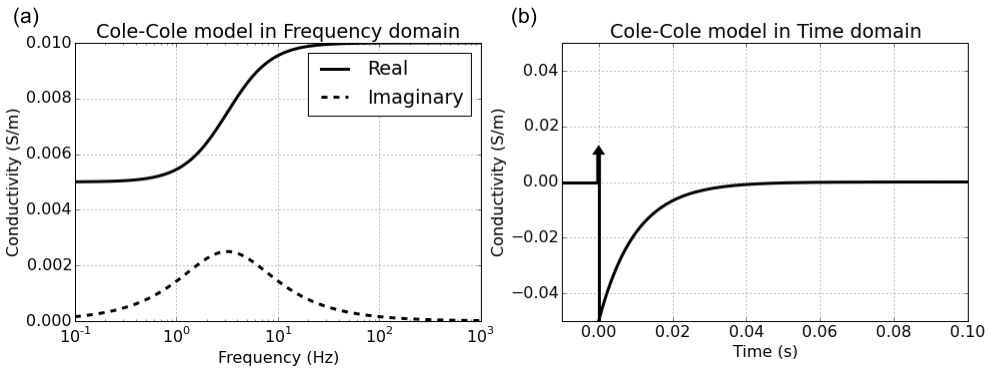
\includegraphics[width=1.0\textwidth]{figures/FDandTDCole.png}
  \caption{Cole-Cole model in frequency domain (a) and time (b) domain. The Cole-Cole parameters are $\siginf$ = $10^{-2}$ S/m, $\eta $ = 0.5, $\tau$ = 0.01, and $c$=1.}
  \label{Fig:FDandTDCole}
\end{figure}

%% =============================================================================
%% Sub section. Decomposition of observed responses
%% =============================================================================

\subsection{Decomposition of observed responses}
\label{sec:Decomposition}
IP effects in the observed data are coupled with EM effects. We need to decompose the observations to isolate data associated only with the IP phenomena.  
Maxwell's equations in the time domain, with a quasi-static approximation, are written as:
\begin{linenomath*}
\begin{equation}
  \curl{\e} = -\frac{\partial \b}{\partial t},
  \label{eq: total_farad}
\end{equation}
\end{linenomath*}
\begin{linenomath*}
\begin{equation}
  \curl{\frac{1}{\mu}\b} - \j= \j_{s},
  \label{eq: total_coulomb}
\end{equation}
\end{linenomath*}
where $\e$ is the electric field ($V/m$), $\b$ is the magnetic flux density ($Wb/m^2$), $\j_{s}$ is the current source ($A/m^2$) and $\mu$ is the magnetic permeability ($H/m$). Here $\j$ is the conduction current ($A/m^2$). In the frequency domain, this conduction current, $\J$ is related to conductivity via Ohm’s law: $\J(\omega) = \sigma(\omega)\E(\omega)$ where $\E$ is the electric field. 
Converting this relationship to time domain using the inverse Fourier transform yields:
\begin{linenomath*}
\begin{equation}
  \j(t) = \sigma(t)\otimes \e(t) = \int_0^t \sigma(u) e(t-u) du.
  \label{eq: ohms_law_convolution}
\end{equation}
\end{linenomath*}
where $\otimes$ indicates time convolution for a causal signal.  
Thus the current density depends upon the previous history of the electric field.
As in \cite{Smith1988a}, we represent total fields as $\e = \e^{F} + \e^{IP}$, $\b = \b^{F} + \b^{IP}$ and $\j = \j^{F} + \j^{IP}$, where superscript $F$ indicates fundamental and $IP$ is induced polarization. 
Here fundamental fields indicate EM fields without IP effects. 
Substituting into eqs (\ref{eq: total_farad}) and (\ref{eq: total_coulomb}) yields the following sequences:
\begin{linenomath*}
\begin{equation}
  \curl({\e^{F}+\e^{IP}}) = -\frac{\partial}{\partial t} (\b^{F}+\b^{IP}),
\end{equation}
\end{linenomath*}
\begin{linenomath*}
\begin{equation}
  \curl\frac{1}{\mu}(\b^{F}+\b^{IP}) - (\j^{F}+\j^{IP})= \j_{s}.
\end{equation}
\end{linenomath*}

The fundmental equations can be written as
\begin{linenomath*}
\begin{equation}
  \curl \e^{F} = -\frac{\partial \b^{F}}{\partial t},
  \label{eq: eq_primary_farad}
\end{equation}
\end{linenomath*}
\begin{linenomath*}
\begin{equation}
  \curl{\frac{1}{\mu}\b^{F}} -\j^{F} = \j_s.
  \label{eq: eq_primary_coulomb}
\end{equation}
\end{linenomath*}
Here
\begin{linenomath*}
\begin{equation}
  \j^{F} = \siginf\e^{F}.
  \label{eq: jF}
\end{equation}
\end{linenomath*}

Substituting the fundamental fields into eqs (\ref{eq: total_farad}) and (\ref{eq: total_coulomb}) yields the expressions for the IP fields 
\begin{linenomath*}
\begin{equation}
  \curl \e^{IP} = -\frac{\partial \b^{IP}}{\partial t},
  \label{eq: eq_secondary_farad}
\end{equation}
\end{linenomath*}
\begin{linenomath*}
\begin{equation}
  \curl{\frac{1}{\mu}\b^{IP}} = \j^{IP}.
  \label{eq: eq_secondary_coulomb}
\end{equation}
\end{linenomath*}

Let $F[\cdot]$ denote operator associated with Maxwell’s equations, and let $d$ denote the observations that include both EM and IP effects. 
Keeping the same notation, we can obtain $d = d^{F} + \dip$, where $d^F$ and $\dip$ are fundamental and IP responses, respectively. 
Based on this, we define the IP datum as 
\begin{linenomath*}
\begin{equation}
  \dip = d - d^{F} = F[\sigma(t)]-F[\siginf].
    \label{eq: IPdatum_syn}
\end{equation}
\end{linenomath*}
Here $F[\siginf]$ corresponds to the fundamental response ($d^F$). 
This subtraction process acts as an EM decoupling process, which removes the EM effects from the measured responses. This is the same procedure that formed the basis of work by \cite{routh2001}. 

\subsection{Polarization currents}
When the electric field is appllied to the chargeable medium in the earth, this medium will have charging and discharging processses. 
Depending on the used exictation mechanism: galvanic or inductve, these charging and discharging processes can have different characteristics. 
To obtain insights about these processes, we focus our attention to currents. Using eq. \ref{eq: sigma_freq}, Ohm's law in frequency domain can be written as 
\begin{equation}
	\J(\omega) = \sigma(\omega)\E(\omega)= \siginf\E(\omega) + \J^{pol}(\omega),
	\label{eq:OhmslawFreq}
\end{equation}
where capital characters denote frequency domain, $\omega$ is angular frequency (rad/s), and the polarization current, $\J^{pol}$ is 
\begin{equation}
	\J^{pol}(\omega) = \dsig(\omega)\E(\omega).
	\label{eq:JpolFreq}
\end{equation}
Applying inverse Fourier transform yields, 
\begin{equation}
	\mathcal{F}^{-1}[\J^{pol}(\omega)] = \j^{pol}(t) = \dsig(t)\otimes \e(t).
	\label{eq:polarization_current}
\end{equation}
From the convolution between $\dsig(t)$ and $\e(t)$, polarization currents can be considered as ``a time record of charging and discharging'' occurring in a chargeable medium due to the applied electric field. 

We consider a situation where a chargeble block is embedded in the half-space earth, and conductivity of the chargeble block is same as that of the half-space which we call canonical model. Both galvanic and inductive sources will be considered. First, for the galvanic source input current waveform ($I(t)$) has constant on and off times as shown in Fig. ~\ref{F:ChargConcept}(a). At an single pixel in the chargeable body, if we measure $x$-component of the fundamental electric field ($e_x^F(t)$), time dependency of that will be exaclty same as $I(t)$. Note that the fundamental fields do not consider any IP effects, and the observations are summation of fundamental and IP fields from eq. ~\ref{eq: IPdatum_syn}. 

On the other hand, for the inductive source, we assume a step-off waveform as shown in Figure ~\ref{F:ChargConcept}(b). Here step-off waveform indicates that we have enough on time that earth medium reaches to the steady state. At that moment, electric field in the earth is zero. This is a funadamental difference of the inductive source to the galvanic source that the earth does not have any steady state electric field. After step off, at the single pixel of the earth, electric field increases from zero, reaches to the peak, then decays as shown in Figure ~\ref{F:ChargConcept}(b).  

To evaluate polarization current, we use assume
\begin{equation}
  \j^{pol}(t) = \dsig(t)\otimes \e^{\ F}(t).
\end{equation}
By convolving $\dsig(t)$ to the fundamental electric fied we obtain polarization current for each source (eq. \ref{eq:polarization_current}). Figure ~\ref{F:jpolDCEM}(a) and (b) shows convolution of $\dsig(t)$ and $\e^F(t)$ for galvanic and inductive sources, respectively. 
Polarization current for the galvanic source, reaches to the steady state, although that for the inductive source does not achieve the steady state, which makes more complicated charging and discharging process for the inductive source. This difference between galvanic and inductive sources should be effectively considered to extract IP information from EM data. 

\begin{figure}  
  \centering
  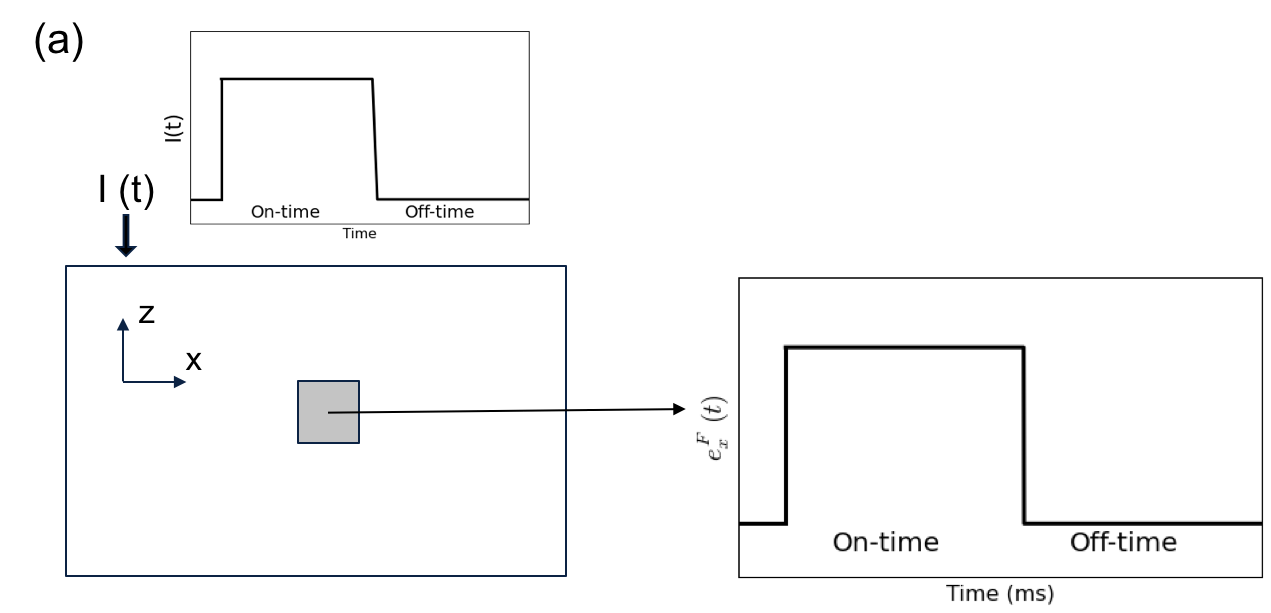
\includegraphics[width=0.6\textwidth]{figures/chargDC.png} \\
  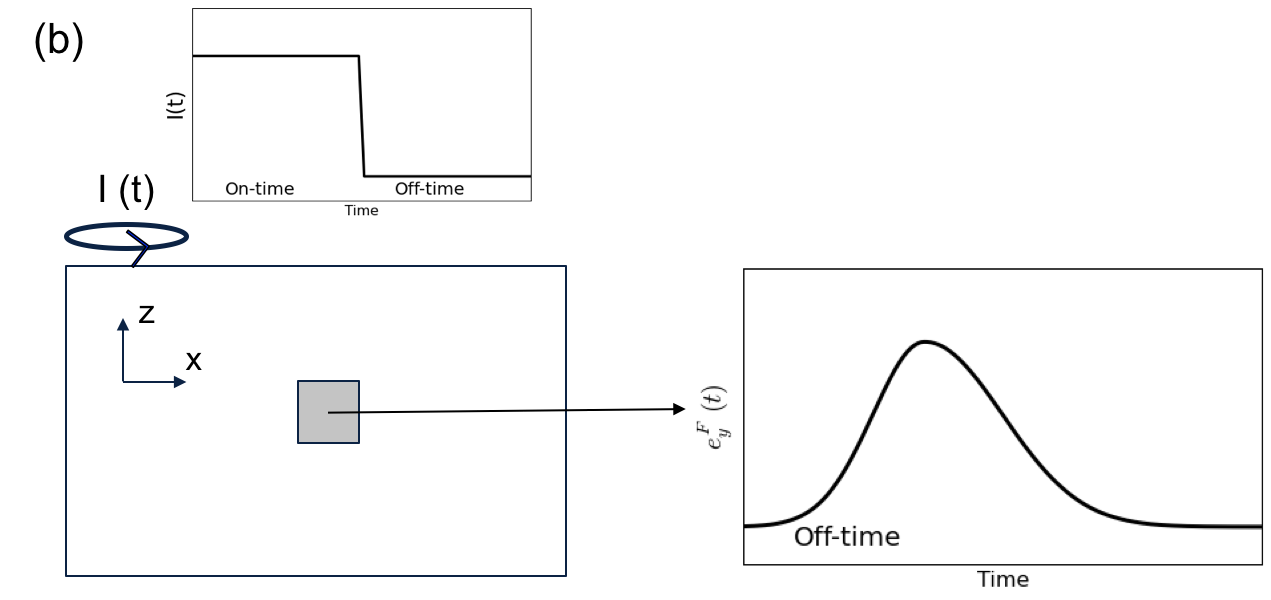
\includegraphics[width=0.6\textwidth]{figures/chargAC.png} 
  \caption{Conceptual diagrams of fundamental electric fields in a chargeable block. (a) Galvanic source and (b) Inductive source. }
  \label{F:ChargConcept}
\end{figure}   

\begin{figure}  
  \centering
  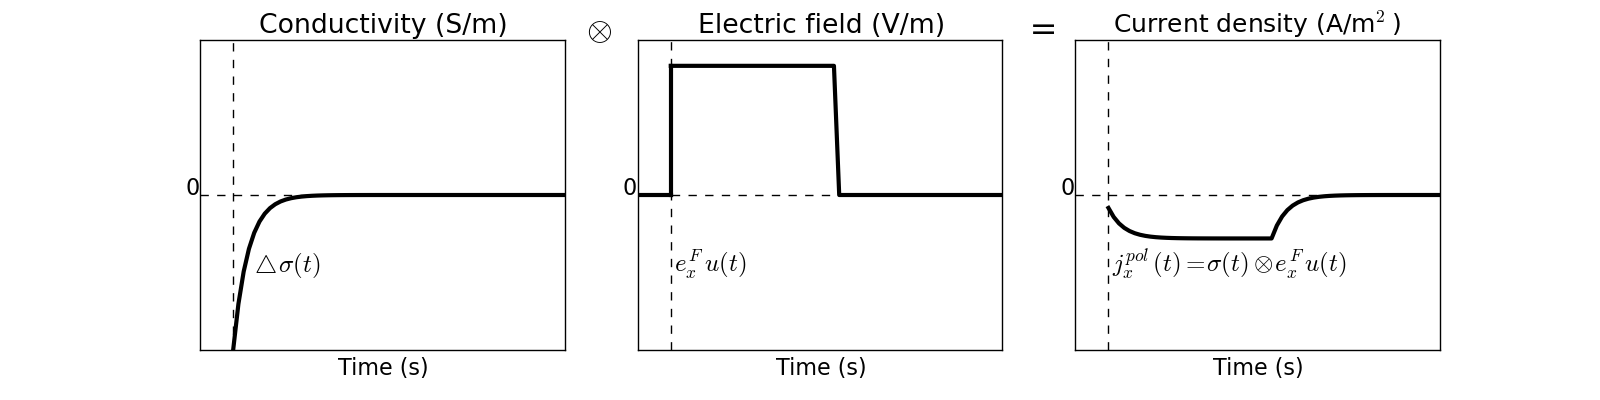
\includegraphics[width=0.9\textwidth]{figures/jpolDC.png}\\ 
  (a) \\
  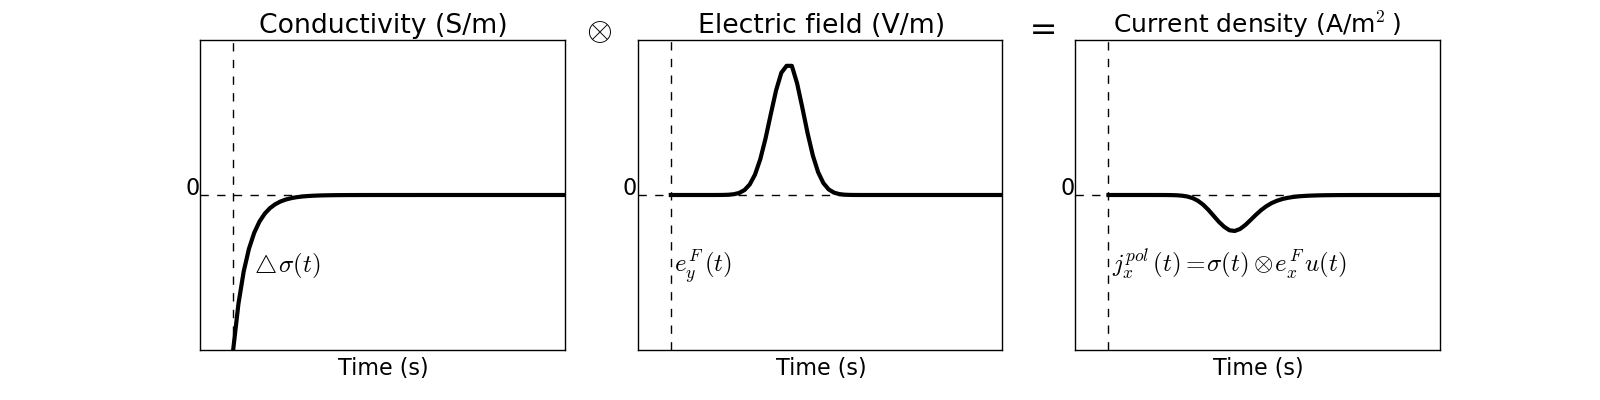
\includegraphics[width=0.9\textwidth]{figures/jpolEM.png} \\
  (b)
  \caption{Polarization current at a single pixel int the chargeable medium. (a) Galvanic and (b) inductive sources.}
  \label{F:jpolDCEM}
\end{figure}   
\clearpage

%%%%%%%%%%%%%%%%%%%%%%%%%%%%%%%%%%%%%%%%%%%%%%%%%%%%%%%%%%%%%%%%%%%%%%%%%%%%%%%%
%% =============================================================================
%% Section. METHODOLOGY
%% =============================================================================
%%%%%%%%%%%%%%%%%%%%%%%%%%%%%%%%%%%%%%%%%%%%%%%%%%%%%%%%%%%%%%%%%%%%%%%%%%%%%%%%

\section{METHODOLOGY}
\section{Pseudo-chargeability}
Combining eqs (\ref{eq: sigma_time}) and  (\ref{eq: ohms_law_convolution}) writing $\j(t)=\j^F + \j^{IP}$ we obtain
\begin{linenomath*}
\begin{equation}
  \j^{IP} = \siginf \e^{IP} + \j^{pol}.
  \label{eq:IP_current}
\end{equation}
\end{linenomath*}
From the previous section, we identified different characteristics of polarization charge builup for the inductive and galvanic sources. 
More specifically, we consider two cases: a) galvanic source without EM induction and b) inductive source with EM induction. The first case corresponds to EIP \cite[]{seigel1959}, and the second is ISIP.
A fundamental difference for these two cases were: 
\begin{itemize}
  \item EIP: the electric field is instantaneous due to the steady-state electric field (Fig. ~\ref{F:ChargConcept} (a)
  \item ISIP:  the electric field in the off-time is not zero, but increases to a peak and then decays as shown in Fig. ~\ref{F:ChargConcept} (b)
\end{itemize}

The polarization current for the two different sources will be significantly affected by these different electric fields as shown in Fig. ~\ref{F:jpolDCEM}. 
To capture this difference in a linearized kernel for the IP response, we define pseudo-chargeability, $\peta(t)$ as 
\begin{linenomath*}
\begin{equation}
  \peta(t) = -\frac{\j^{pol}(t)}{\j^{\ ref}},
  \label{eq:pseudochargeability_0}
\end{equation}
\end{linenomath*}
where the reference current ($\j^{ref}$) is defined as 
\begin{linenomath*}
\begin{equation}
  \j^{\ ref} = \siginf \eref.
  \label{eq:reference_current}
\end{equation}
\end{linenomath*}
Here $\eref$ is the reference electric field and both $\j^{\ ref}$ and $\eref$ are static fields that are independent of time. 
The pseudo-chargeability defined in eq. (\ref{eq:pseudochargeability_0})  is the ratio of  the polarization current to the reference current. This is a small quantity and it plays an essential role in our linearization. 

To evaluate the pseudo-chargeability, we have to identify the reference current or reference electric fields. For the EIP case, the electric field, when there is no IP present, is independent of time as shown in Fig. \ref{F:DCEM_F_current}(a). For the inductive source however, the electric field does not achieve a steady-state, but increases to a  peak then decreases. 

Each pixel in the earth has its own reference electric field and time thus  both $\eref$ and $t^{\ ref}$ have a 3D distribution. 
For both EIP and ISIP cases, we mathematically present our choice of the reference electric field as
\begin{linenomath*}
\begin{equation}
  \eref = \e^{F}(t) \otimes \delta(t-t^{\ ref}). 
  \label{eq:reference_electricfield}
\end{equation}
\end{linenomath*}
The reference time for the EIP case can be any time in the on-time, because the fundamental electric field for the EIP case does not change in on-time. 

By rearranging eq. (\ref{eq:pseudochargeability_0}), we obtain 
\begin{linenomath*}
\begin{equation}
  \j^{pol} = -\jref\peta(t). 
  \label{eq:polarization_current_concept}
\end{equation}
\end{linenomath*}
This states that the polarization current has an opposite direction to the reference current, and is proportional to the pseudo-chargeability ($\peta(t)$). 
This conceptual model about the polarization current shown in eq. (\ref{eq:polarization_current_concept}) is consistent with \cite{seigel1959}'s result. We note, that for any pixel, even though  $\eref$  attains the same value for an ISIP survey as for an EIP survey, the pseudo-chargeability resulting from  an ISIP survey  will be less than that from an EIP survey. We can infer from this that  linearization techniques, which  have worked so well in EIP problems, should be successful in ISIP problems. 
\begin{figure}  
  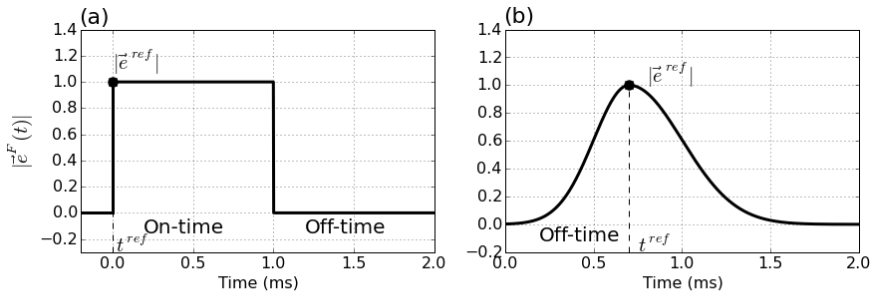
\includegraphics[width=1.0\textwidth]{figures/DCEM_F_current.png} 
  \caption{Conceptual diagram for the amplitude of the fundamental electric fields. (a) EIP and (b) ISIP cases.}
  \label{F:DCEM_F_current}
\end{figure}   

\subsection{Linearization}
Following from the methodologies in EIP, our goal is to express the IP response ($\dip$) as a function of the pseudo-chargeability $(\peta(t))$ in time  $\dip(t) = J[\peta(t)]$, where $J[\cdot]$ is a linear operator which is independent of time. In doing this we first consider a general EM system which is applicable to galvanic or inductive sources. 
For any pixel  volume in the earth the amplitude and direction of the  electric field can vary dramatically  in time and this results in a complicated  IP charging process. If substantial polarization currents are developed however, they will correspond to a maximum electric field or reference current aligned in a constant direction. Our formulation focuses on this aspect. We assume that the final large-scale IP response observed in the data is the result of  pixels being charged with an electric field in a specific direction but with a variable amplitude. Let $\e(t)$ be approximated as
\begin{linenomath*}
\begin{equation}
  \e(t) \approx \eref \hat{w}(t),
  \label{eq: e_with_eref}
\end{equation}
\end{linenomath*}
where $\hat{w}(t)$ is defined as:
\begin{linenomath*}
\begin{equation}
  \hat{w}(t) = P_0[w^{ref}(t)].
  \label{eq: we}
\end{equation}
\end{linenomath*}
Here a projection ($P_0[\cdot]$) of an arbitrary function, $f(t)$ is
\begin{linenomath*}
\begin{equation}
  P_0[f(t)] = \left\{ 
  \begin{array}{l l}
    f(t) & f(t) \ge 0 \\
    0 & \text{if } f(t) < 0, 
  \end{array}\right.
  \label{eq: P0}
\end{equation}
\end{linenomath*}
and
\begin{linenomath*}
\begin{equation}
  w^{ref}(t) = \frac{\e^F(t)\cdot\eref}{\eref\cdot\eref}.
  \label{eq: wref}
\end{equation}
\end{linenomath*}
Here $w^{ref}(t)$ is a dimensionless function that prescribes the time history of the electric field at each location along the direction of the chosen reference electric field ($\eref$).  Negative values of  $w^{ref}(t)$ are set to zero in accordance with our conceptual model that polarization currents have an opposite direction to the reference current (eq. \ref{eq:polarization_current_concept}).
We redefine the pseudo-chargeability as
\begin{linenomath*}
\begin{equation}
    \peta(t) = \peta^{I}(t)\otimes \hat{w}(t).
    \label{eq: pseudochargeability}
\end{equation}
\end{linenomath*}
The polarization current, $\j^{pol}$ can be approximated with eq. (\ref{eq: intrinsic_peta}) as
\begin{linenomath*}
\begin{equation}
  \j^{pol}(t) \approx - \peta^{I}(t)\otimes \hat{w}(t)\jref.
\end{equation}
\end{linenomath*}
Substituting this into eq. (\ref{eq:IP_current}) yields
\begin{linenomath*}
\begin{equation}
  \j^{IP}(t) \approx \siginf\e^{IP}(t) - \peta^{I}(t)\otimes \hat{w}(t)\jref
\end{equation}
\end{linenomath*}
and this yields
\begin{linenomath*}
\begin{equation}
  \j^{IP}(t) \approx \siginf\e^{IP}(t) -\jref\peta(t).
  \label{eq: jip_EMIP}
\end{equation}
\end{linenomath*}

The second term, $-\jref\peta(t)$, correspond to polarization currents. The first term, $\siginf \e^{IP}(t)$ is usually omitted \cite[]{Smith1988a}. Here we include it and explore the conditions in which it is important. 
Because the reference current is static, any time-dependency in the polarization currents is encapsulated in the pseudo-chargeability. The buildup and decrease of polarization currents is a slow process and we assume therefore that this process does not produce induction effects ($\frac{\partial \b^{IP}}{\partial t} \approx 0$) and hence we can write 
\begin{linenomath*}
\begin{equation}
  \e^{IP} \approx  \e^{IP}_{approx} = -\grad\phi^{IP}.
  \label{eq: eip_approx}
\end{equation}
\end{linenomath*}

By taking the divergence of  eq. (\ref{eq: jip_EMIP}), substituting  $\e^{IP}$ with eq. (\ref{eq: eip_approx}), and carrying out some linear algebra, we obtain
\begin{linenomath*}
\begin{equation}
  \phi^{IP}(t) \approx -[\div \siginf\grad]^{-1}\div\jref\peta(t).
  \label{eq: phiIPapprox_general}
\end{equation}
\end{linenomath*}
By applying the gradient we obtain 
\begin{linenomath*}
\begin{equation}
    \e^{IP}_{approx} = \grad[\div \siginf\grad]^{-1}\div\jref\peta(t).
    \label{eq: eip_approx_full}
\end{equation}
\end{linenomath*}
Thus, the electric field due to the IP effect can be expressed as a function of $\peta(t)$ in time. 
This form is also applicable to the  EIP case.   

For an inductive source, the data is often either $\b$ or its time derivative and hence we also need to compute $\b^{IP}$ or its time derivative.
For this, we first compute $\j^{IP}$ then use the Biot-Savart law. 
By substituting eq. (\ref{eq: eip_approx_full}) into eq. (\ref{eq: jip_EMIP}), the approximated IP current density, $\j^{IP}_{approx}$ can be expressed as
\begin{linenomath*}
\begin{equation}
  \j^{IP}(t) \approx \j^{IP}_{approx} = \bar{S}\jref\peta(t),
  \label{eq: jip_approx}
\end{equation}
\end{linenomath*}
where
\begin{linenomath*}
\begin{equation}
  \bar{S} = \siginf\grad[\div \siginf\grad]^{-1}\div-\bar{I}
\end{equation}
\end{linenomath*}
and $\bar{I}$ is an identity tensor. 
Applying the Biot-Savart law we have:
\begin{linenomath*}
\begin{equation}
  \b^{IP}_{approx}(\vec{r}; t) = \frac{\mu_0}{4\pi}\int_{\Omega}  \frac{\bar{S}\j^{\ ref}(\vec{r}_s)\times\hat{r}}{|\vec{r}-\vec{r}_s|^2}\peta(t)d\vec{r}_s,
  \label{eq: BiotbIP_approx}
\end{equation}
\end{linenomath*}
where $\vec{r}_s$ indicates a vector for a source location, and $\hat{r}=\frac{\vec{r}-\vec{r}_s}{|\vec{r}-\vec{r}_s|}$.
If $\siginf\e^{IP}$ is omitted in  $\j^{IP}$ then the tensor, $\bar{S}$ becomes $-\bar{I}$. 
In this situation, the IP current is same as the polarization current, and it always has opposite direction to the reference current. 
This reversed current, along with Biot-Savart law,  provides a physical understanding about the negative transients in ATEM data when the earth is chargeable. 

Observed data are often the time derivative of $\b$, hence by taking time derivative to the eq. (\ref{eq: BiotbIP_approx}), we obtain
\begin{linenomath*}
\begin{equation}
  -\frac{\partial\b^{IP}_{approx}}{\partial t}(\vec{r}; t) = \frac{\mu_0}{4\pi} \int_{\Omega}  \frac{\bar{S}\jref(\vec{r}_s)\times\hat{r}}{|\vec{r}-\vec{r}_s|^2} \Big( -\frac{\partial \peta(t)}{\partial t} \Big) d\vec{r}_s.
  \label{eq: BiotbIPdt_approx}
\end{equation}
\end{linenomath*}
Here we have chosen to keep the minus signs in eq. (\ref{eq: BiotbIPdt_approx}) so that $-\frac{\partial \peta(t)}{\partial t}$ is positive when $\peta(t)$ is decaying in time. 
Accordingly, the IP datum is given by  $-\frac{\partial\b^{IP}}{\partial t}$. 

The IP fields shown in eqs (\ref{eq: eip_approx_full}), (\ref{eq: BiotbIP_approx}) and (\ref{eq: BiotbIPdt_approx}) are linear functionals of $\peta$ and the equations for a single time channel can be discretized in space as
\begin{linenomath*}
\begin{equation}
  \mathbf{d}^{IP} = \mathbf{J}\peta,
  \label{eq: dIP_lineareq}
\end{equation}
\end{linenomath*}
where $\mathbf{J}$ is the corresponding sensitivity matrix. 
In particular when the observed datum is the time derivative of $\b$, the linear relationship can be written as 
\begin{linenomath*}
\begin{equation}
  \mathbf{d}^{IP} = \mathbf{J}(-\frac{\partial \peta}{\partial t}\Big|).
  \label{eq: dIP_lineareq_dbdt}
\end{equation}
\end{linenomath*}
The representation in eq. (\ref{eq: dIP_lineareq}) is valid for galvanic and inductive sources but the two assumptions: a) $\e \approx \eref \hat{w}(t)$ and b) $\e^{IP} \approx -\grad\phi^{IP}$ need to be tested numerically for the case of inductive sources. 

\subsection{Handling multiple transmitters in ATEM surveys}
\label{subsection: Handling multiple transmitters in ATEM surveys}
The work for inductive sources in the previous sections has been developed for a single transmitter and 3D information about chargeability can be obtained if there are multiple receivers. For ATEM data however, we have only a single receiver location for each transmitter but we have multiple transmitter locations. 
Our goal is to alter the problem to work with an effective pseudo-chargeability. 

In our linearized eq. (\ref{eq: dIP_lineareq}), each transmitter has its own sensitivity and pseudo-chargeabilty. For our airborne case the sensitivity for the $k$-th transmitter is the $k$-th row of $\mathbf{J}$ and the pseudo-chargeability is $\peta^k$. The corresponding  IP datum is 
\begin{linenomath*}
\begin{equation}
  \dip_k(t) = \sum_{i=1}^{nC}J_{k,i}\peta^k_i (t), \ \ k=1, \ldots, nTx,
  \label{eq: dip_kthTx}
\end{equation}
\end{linenomath*}
where $nTx$ is the number of transmitters, $nC$ is the number of cells in the domain, and $J_{k,i}$ indicates an element of the Jacobian matrix for the $k$-th transmitter and the $i$-th cell. We want to replace $\peta^k_i$ with a single effective pseudo-chargeabilty $\peta^k$ and therefore write the IP datum as 
\begin{linenomath*}
\begin{equation}
  \dip_k(t) = \sum_{i=1}^{nC}J_{k,i}\peta_i (t), \ \ k=1, \ldots, nTx,
  \label{eq: dipeff_kthTx}
\end{equation}
\end{linenomath*}
The waveforms are different for each transmitter and hence this representation cannot be exact. To examine the implications of this it suffices to look at the contribution of any volumetric pixel. Each pixel contributes to all of the IP data but in differing amounts. The total contribution of the  $i$-th pixel to the $nTx$ data set at a single time is  
\begin{linenomath*}
\begin{equation}
  q_i =\sum_{k=1}^{nTx} J_{k,i} \peta^k_i(t), \ \ i=1, \ldots, nC.
  \label{eq: dip_hat}
\end{equation}
\end{linenomath*}
Our goal is to find an effective chargeability that produces the same net effect on the measured data. We search for a transmitter-independent $\peta_i$ such that 
\begin{linenomath*}
\begin{equation}
  q_i^{est} =\sum_{k=1}^{nTx} J_{k,i} \peta_i(t), \ \ i=1, \ldots, nC.
  \label{eq: dip_tilde}
\end{equation}
\end{linenomath*}
Minimizing the least squares difference between eqs (\ref{eq: dip_hat}) and (\ref{eq: dip_tilde}) yields
\begin{linenomath*}
\begin{equation}
  \peta_i(t) = \frac {\Sigma_{k=1}^{nTx} J_{k,i}^2\peta^k_i(t)} {\Sigma_{k=1}^{nTx} J_{k,i}^2} = \sum_{k=1}^{nTx} a^k_i \peta^k_i(t), \ \ i=1, \ldots, nC.
  \label{eq: petaeff}
\end{equation}
\end{linenomath*}
where normalized weight ($a^k_i$) is 
\begin{linenomath*}
\begin{equation}
  a^k_i = \frac {J^2_{k,i}} {\Sigma_{k=1}^{nTx} J^2_{k,i}}, \ \ i=1, \ldots, nC.
  \label{eq: normalized_weights}
\end{equation}
\end{linenomath*}

With the above understanding about how $\peta_i$ relates to the $\peta_i^k$ from each transmitter we can proceed  as follows. Firstly, from eq. (\ref{eq: pseudochargeability}) we have 
\begin{linenomath*}
\begin{equation}
  \peta_i^k(t) =\peta^I \otimes \hat{w}^{k}_i(t) 
  \label{eq: peta_transmitters}
\end{equation}
\end{linenomath*}
Substituting eqs (\ref{eq: peta_transmitters}) into (\ref{eq: petaeff}) allows us to write
\begin{linenomath*}
\begin{equation}
  \peta_i(t) = \peta^I(t) \otimes w^e_i(t),
\end{equation}
\end{linenomath*}
where we define effective time history of the electric field, $w^e_i(t)$ as 
\begin{linenomath*}
\begin{equation}
  w^e_i(t)= \sum_{k=1}^{nTx} a^k_i \hat{w}^{k}_i(t), \ \ i=1, \ldots, nC.
  \label{eq: we_eff}
\end{equation}
\end{linenomath*}

The above equations shows that the pseudo-chargeabilty for any pixel recovered from the inversion is equal to the convolution of the intrinsic pseudo-chargeability ($\peta^I(t)$) with an effective time history of the electric field ($w^e(t)$). Although it is somewhat involved, the $w^e(t)$ associated with each pixel can be evaluated by knowing the electric fields associated with the fundamental EM problem. Ultimately this allows us to estimate the parameters associated with the intrinsic pseudo-chargeability in the same manner as outlined for the case with a single transmitter. 
%%% ===========================================================================
%%% SUBSECTION
\subsection{3D IP inversion with a linearized kernel}
The linear inverse problem to recover chargeability is straightforward and is described in \cite{doug1994}. 
We rewrite eq. (\ref{eq: dIP_lineareq}) as
\begin{linenomath*}
\begin{equation}
  \mathbf{d}^{pred} = \mathbf{J}\mathbf{m},
  \label{eq9}
\end{equation}
\end{linenomath*}
where $\mathbf{J}$ is the  sensitivity matrix of linear problem, which corresponds to $\mathbf{J}$ shown in eq. (\ref{eq: dIP_lineareq}). 
Here, $\mathbf{d}^{pred}$ represents IP responses at a single time channel, $\mathbf{m}$ denotes model parameters, which can be either $\peta$ or $-\frac{\partial \peta}{\partial t}\big|$ at the same time. 
In our work here we invert each time channel of $d^{IP}$, separately. 

The solution to the inverse problem is the model $\mathbf{m}$ that solves the optimization problem
\begin{linenomath*}
\begin{equation}
  minimize \ \phi =  \phi_d(\mathbf{m}) + \beta\phi_m(\mathbf{m}) \\
  s.t. \ 0 \le \mathbf{m},
  \label{eq10}
\end{equation}
\end{linenomath*}
where $\phi_d$ is a measure of data misfit, $\phi_m$ is a user-defined model objective function and $\beta$ is regularization or trade-off parameter. We solve this optimization problem using a projected Gauss-Newton method \cite[]{Kelley}. 
The value of $\beta$ is determined using a cooling technique where $\beta$ is progressively reduced from some high value. The inversion is stopped when the tolerance is reached (cf. \cite{DougTutorial, Kang2014}). 

We use the sum of the squares to measure data misfit
\begin{linenomath*}
\begin{equation}
  \phi_d = \| \mathbf{W_d}(\mathbf{A}\mathbf{m}-d^{obs}|)\|^2_2 =
  \sum^N_{j=1}(\frac{\mathbf{d}^{pred}_j-\mathbf{d}^{obs}_j}{\epsilon_j}),
  \label{eq11}
\end{equation}
\end{linenomath*}
where $N$ is the number of the observed data and $\mathbf{W_d}$ is a diagonal data weighting matrix which contains the reciprocal of the estimated uncertainty of each datum ($\epsilon_j$) on the main diagonal,  $\mathbf{d}^{obs}$ is a vector containing the observed data, $\mathbf{d}^{pred}$ is a vector containing calculated data from a linear eq. given in eq. (\ref{eq9}).
The model objective function, $\phi_m$, is a measure of the amount structure in the model and upon minimization this will generate a smooth model which is close to a reference model, $m_{ref}$. 
We define $\phi_m$ as
\begin{linenomath*}
\begin{equation}
  \phi_m = \sum_{i=s,x,y,z} \alpha_i\| \mathbf{W}_i\mathbf{W}(\mathbf{m}-\mathbf{m}_{ref})\|^2_2,
  \label{eq12}
\end{equation}
\end{linenomath*}
where $\mathbf{W}_s$ is a diagonal matrix, and $\mathbf{W}_x$, $\mathbf{W}_y$ and $\mathbf{W}_z$ are discrete approximations of the first derivative operator in $x$, $y$ and $z$ directions, respectively.  
The $\alpha$'s are weighting parameters that balance the relative importance of producing small or smooth models, and $\mathbf{W}$ stands for model weighting matrix \cite[]{LiMag3D}.

\subsection{IP inversion procedure}
As seen in the previous sections the extraction of IP information from TEM data has multiple steps. These include: (1) invert TEM data and recover a 3D conductivity model ($\sigma_{est}$). 
(2) Forward model $\sigma_{est}$ to obtain the fundamental response $d^F$ and subtract it from the observations to obtain $\dip$ data.
(3) Consider a possible regional fields from the subtraction due to incorrect conductivity model, and remove.
(4) Invert  $\dip$ data to recover pseudo-chargeability model at individual time channels using the relationship in eq. (\ref{eq: dIP_lineareq}). 
(5) Further, process the inversion outputs at multiple time-channels  to estimate the Cole-Cole, or equivalent IP parameters.
Figure ~\ref{F:IPprocedure} shows above IP inversion procedure as a flow chart. 
In the following we investigate each of the above steps via numerical simulations and test the validity of our assumptions. 
\begin{figure}  
  \centering
  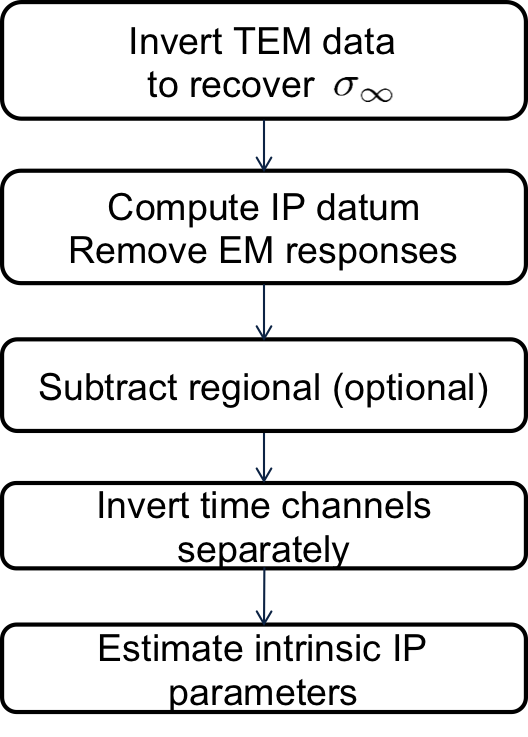
\includegraphics[width=0.4\textwidth]{figures/IPprocedure.png} 
  \caption{A flow chart of the IP inversion procedure.}
  \label{F:IPprocedure}
\end{figure}   


\section{REVISITING ELECTRICAL IP}
To extract IP information from the EIP data in time domain, convetionally, we first estimates the background conductivity from the asymptotic on-time data and then inverts off-time data to recover information about ``chargeability'' \cite[]{doug1994}. 
A fundamental assumption behind this approach is that Electromagnetic (EM) induction phenomenon is ignored. 
This assumption obviously does not make sense whenever there are siginficant EM induction effect in the observation. Likely, this can happen at earlier times or when the earth medium is significatly conductive. 
This effect is often called “EM coupling”, because our interest is mostly in IP signals. Even in the early days of IP method, people recognized that EM coupling can be significant, and tried to decouple them using simple Tx-Rx geometry and model (i.e., half-space model). Although this approach might be effective for certain cases where this simple model is close to the ground truth, obviously there can be a number of situations where this does not make sense. 

By using our capability of 3D simulations and inversions \cite[]{Marchant2014,Li2000,Chen2003}, we systematically revisit this assumption for both EIP and MIP problems, and clearly identify when and what circumstances this assumption breaks. Then we apply our IP procedure to the observed data including both EM and IP responses to extract distributed IP information. This has not been throughly investigated yet but will be . 

\section{VALIDATION OF LINEARIZATION}
Each step of our linearization approach should be carefully validated for different IP applications in. We have tested our linearization approach and suggested its validity for ISIP case, and this will be the basement of following sections. Although this part is an essential elements of our Ph.D. research, we omitted in this proposal to focus on more practical examples. We have submitted an article about this validation (\cite{Kang2015c}).

\section{AIRBORNE IP}
Airborne EM (AEM) systems use inductive source, which excite the earth using EM induction phenomenon. Therefore different from EIP, we cannot simply ignore EM induction effect for airborne IP. Espeically for time domain systems using coincident-loop geometry, negative transients has been observed in the field survey, which cannot be explained by any time-independent conductivity structure. \cite[]{Weidelt1982} showed that IP effect can be a most plausible candidate to explain negative transients. There are few important questions that has not been clearly answered about airborne IP:
\begin{enumerate}
  \item Can we identify IP responses embedded in the EM response?
  \item Can we recover 3D IP information?
  \item How deep IP target can be detected using current AEM system?
  \item What is the source of the IP?  
\end{enumerate}
We focus on first two questions in following examples, but other items will be investigated on our Ph.D. research. 
\subsection{Synthetic example}
To investigate the suggested IP inversion methodology to recover distributed IP information from airborne time domain EM (ATEM) data, we compose an synthetic Cole-Cole model in 3D assuming $c$=1. $\siginf$ model is shown in Fig. \ref{Fig:condandetamodel}. Conductivities of the background and conductive overburden on west side are $10^{-3}$ and $10^{-3}$ S/m, respectively. We have four IP bodies, which named A1-A4. Those four bodies have different $\siginf$ and $\eta$ values as shown in Table \ref{Table: properties}. $\eta$ values except for those IP bodies are set to 0, and $\tau$ is fixed to 0.005 for all IP bodies. To compute synthetic ATEM data from this Cole-Cole model, we use EMTDIP code developed by (\cite{Marchant2014}). Survey geometry includes 21 lines as shown in the top-left panel of Fig. \ref{Fig:condandetamodel} as black dots. We use coincident-loop system and both transmitter and receiver are located 30 m above the surface; radius of the loop is 10 m. Step-off waveform is used and the range of time channel is 0.01-10ms. Measured responses is vertical component of $\dbdt$. 

For the IP inversion, we apply a depth weighting through model weighting matrix ($\mathbf{W}$):
\begin{linenomath*}
\begin{equation}
    \mathbf{W} = \mathbf{diag}(\mathbf{z-z_0})^{1.5},
    \label{eq: weight_mat}
\end{equation}
\end{linenomath*}
where $\mathbf{z}$ and $\mathbf{z_0}$ are discretized depth locations and reference depth in the 3D domain. Because we are inverting each time channel of $\dip$ datum, separately, we may not have intrinsic depth resolution similar to the magnetic inversion \cite[]{LiMag3D}. This could be overcome if there were multiple receivers for each transmitter, although usual ATEM surveys only have a single receiver.

In this section, we first estimate $\siginf$ model by applying 3D ATEM inversion to the observed data with exception of IP-contaminated responses. Using this estimated conductivity model, second, we apply the EM decoupling process and compute IP datum. Finally, we apply 3D IP inversion to these IP responses, and restore pseudo-chargeability model. 

\begin{figure}[htb]
  \centering
  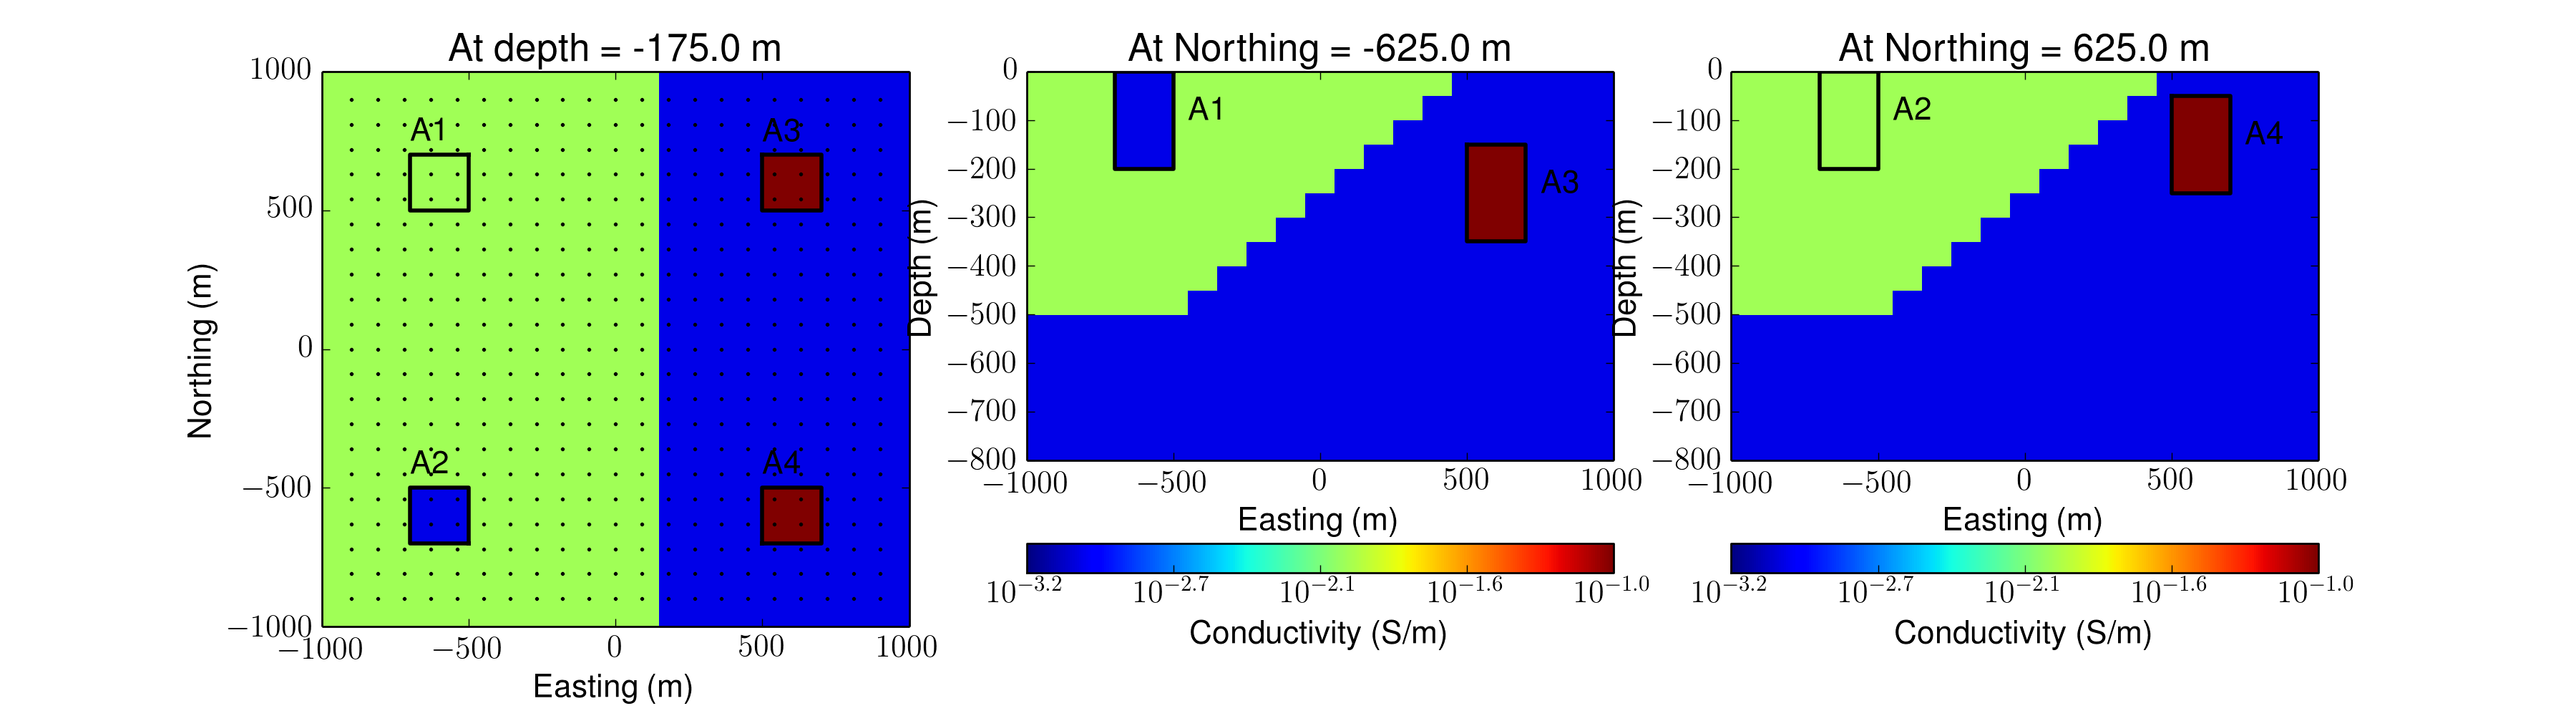
\includegraphics[width=1.0\textwidth]{figures/sigma_Inf.png}
  \caption{Sectional views of 3D $\siginf$ model. Solid lines delineate boundaries of four IP bodies.}
  \label{Fig:condandetamodel}
\end{figure}

\begin{table}[ht]
\caption{Cole-Cole parameters of four anomalous boides (A1-A4). } % title of Table
\begin{center}
  \begin{tabular}{ |c|c|c|c|c|c| } 
  \hline
  Division & A1 & A2 & A3 & A4 \\
  \hline
  $\siginf$ (S/m) & $10^{-1}$ & $10^{-3}$ & $1$   & $1$  \\ 
  $\eta $         & 0.5       & 0.5       & 0.4   & 0.8  \\ 
  $\tau$          & 0.005     & 0.005     & 0.005 & 0.005\\ 
  \hline
  \end{tabular}

\end{center}
\label{Table: properties}  
\end{table}
\subsection{EM decoupling}
\label{subsec:emdecoupling}
IP responses are embedded in the observed ATEM responses. Those are coupled with responses due to EM induction, which we named fundamental responses. Therefore, the first step to recover distributed IP information should be decoupling IP responses from fundamental responses. Assuming that we know true $\siginf$ model, this can be simple a subtraction process as shown in equation (\ref{eq: IPdatum_syn}). However, the this assumption can be critical because we do not know this $\siginf$ model. Fortunately, we still have some chances to reasonably restore 3D distribution of $\siginf$ by applying 3D ATEM inversion with exception of IP-contaminated responses. Fig. \ref{Fig:ObsPredIPResp}(a) show the observed responses on all sounding locations at 0.06, 1.25 and 7.65ms. This include both EM induction and IP effects. At earlier time channel (0.06 ms), EM induction is dominant. In contrast, IP gets dominant as we go later time channels (1.25 and 7.65 ms) given that those show negative values near chargeable bodies. To ignore these IP-contaminated responses in our 3D ATEM inversion, we only used time channels ranging from 0.1-1 ms for all soundings, which do not have any negative transient. We used efficient 3D ATEM inversion algorithm \cite[]{yang20143} to recover $\siginf$ model. The estimated $\siginf$ ($\sigma_{est}$) model shown in Fig. \ref{Fig:condestmodel} can be compared to the true $\siginf$ in Fig. \ref{Fig:condandetamodel}. Regional trend and isolated conductive or resistive bodies are well-recovered except for A3, which has the deepest depth of burial. Poor conductivity recovery of A4 shows a possible limitation of our approach: resolving conductivity of deeper target can be challenging because later time channels may be more contaminated by IP effects. 

Using this conductivity model ($\sigma_{est}$), we compute predicted EM respones ($d[\sigma_{est}]$). 
At 0.06 ms, $d$ and $d[\sigma_{est}]$ matches well as shown in Figure ~\ref{Fig:ObsPredIPResp}, whereas they show considerable difference at both 1.25 and 7.65 ms due to the IP effects at those later times. Because $d[\sigma_{est}]$ is not excactly same as $d^{F} = d[\siginf]$, this raw IP datum, $\dip_{raw}$ may include some errors. To examine these more closely we write
\begin{equation}
  \dip_{raw}(t) = d(t) - d[\sigma_{est}](t) = \dip(t) + \triangle d[\siginf](t) + n(t),
  \label{eq: IPdatum_obs}
\end{equation}
where $\dip$ is the true IP data, $n$ is additive noise, and $\triangle d[\siginf]$ ($=d^{F}-d[\sigma_{est}]$) is the error caused because of poor estimate of $\siginf$. 
Undoubtedly there are situations where the errors on the right hand side can become larger than $\dip$. This will always occur at early time channels where IP response is small and EM induction response is large. 
Thus there is an ``earliest'' time channel than can be used for this analysis. 
The second issue concerns $\triangle d[\siginf]$. 
This is more difficult to quantify and needs to be treated on a case-by-case basis. 
It is least important when dealing with resistive bodies and hosts, and most problematic as the bodies and hosts become more conductive. 
There are a few items of note however. 
Firstly, if $\sigma_{est}$ is incorrect by a scale factor then this shifts the $\dip$ data. 
Away from chargeable bodies the $\dip$ response should be zero. 
Assuming these locations can be recognized then the regional shift can be estimated and applied to $\dip_{raw}$. 
The same idea is applicable to long wavelength spatial components of regional fields ($\triangle d[\siginf]$). Any corrective procedure, which is akin to removal of regional fields in potential fields processing, relies on identification of areas in the model believed to be free of IP responses. 

Computed $\dip_{raw}$ is shown in Fig. \ref{Fig:ObsPredIPResp}(c). This clearly shows our EM decoupling gets more effective as we go later times when the strength of $\dip$ considerable to that of $d^F$. In addition, we provided decaying curves at four sounding locations shown in Fig. \ref{Fig:transientsall}. Black dotted line, which indicates negative values in the observed response shows up on late times. 
By inverting some earier times of data when IP effect is minor, we recovered $\sigma_{est}$, and computed $d[\sigma_{est}]$ (solid blue circles). $d[\sigma_{est}]$ shows good match with $d^F$ (blue lines). 
Computed $\dip_{raw}$ (red circles) converges to $\dip$ as we go later times (red lines).
Therefore, the subtraction process in equation (\ref{eq: IPdatum_obs}) shows us good performance after certain later times when $\dip$ is relatively considerable compared to $d^F$, whereas it shows poor performance on early times when $d^F$ is dominant. From this numerical experiment, we can classify three time ranges about EM decoupling:
\begin{enumerate}
  \item No hope: Early time when $|d^F| \gg |\dip|$ ($\sim$ 0.06 ms)
  \item Effective: Intermediate time when $|d^F| \approx |\dip|$ ($\sim$ 1.25 ms)
  \item No need: Late time when $|d^F| \ll |\dip|$ ($\sim$ 7.65 ms)
\end{enumerate}

An ideal case of our EM decoupling approach is when we have enough early times (less contaminated by IP) which includes information of conductivity structures that we are interested. However, in practice, there can be more challenging situation. For instance, the observed data can be completely contaminated by IP even at the earliest time channels. Clearly, we cannot apply our EM decoupling procedure although EM decoupling may not be required. Classification of different types of EM decoupling connected to IP inversion should be systematically laid out.

\begin{figure}[htb]
  \centering
  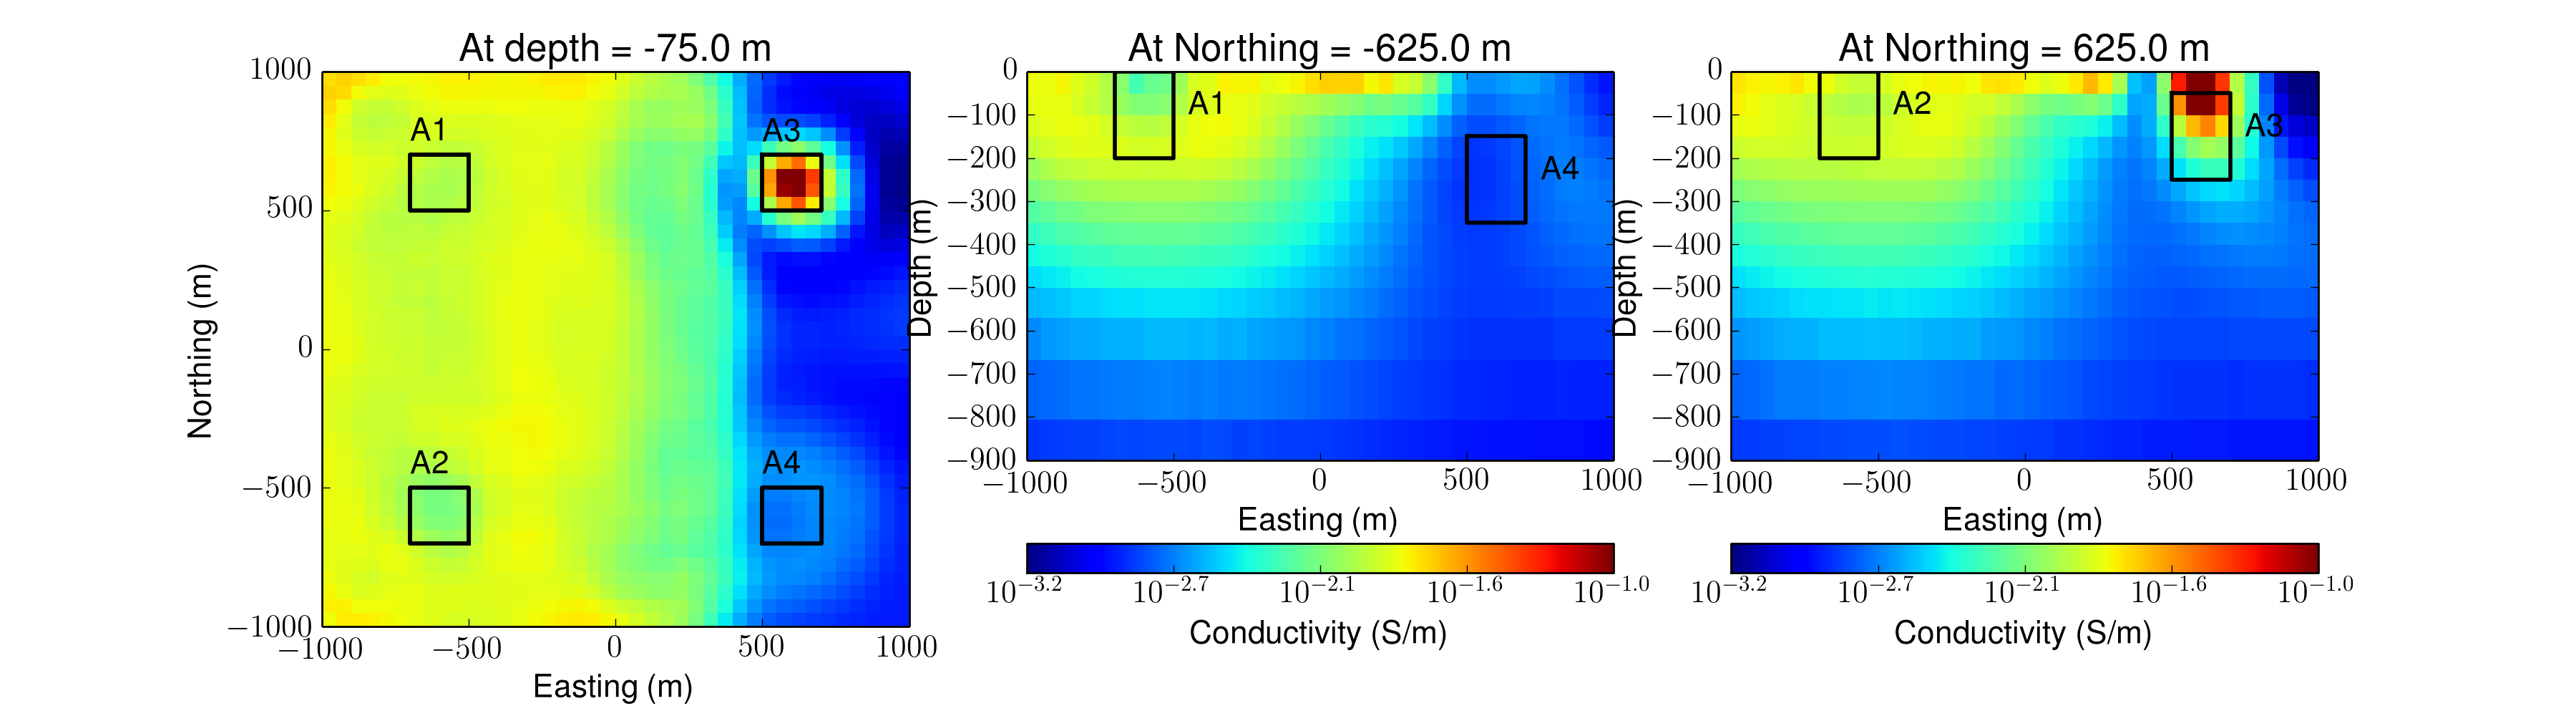
\includegraphics[width=1.0\textwidth]{figures/sigma_est.png}\\(a)
  \caption{Sectional views of the recovered $\siginf$ model ($\sigma_{est}$) from 3D ATEM inversion.}
  \label{Fig:condestmodel}
\end{figure}

\begin{figure}[htb]
  \centering
  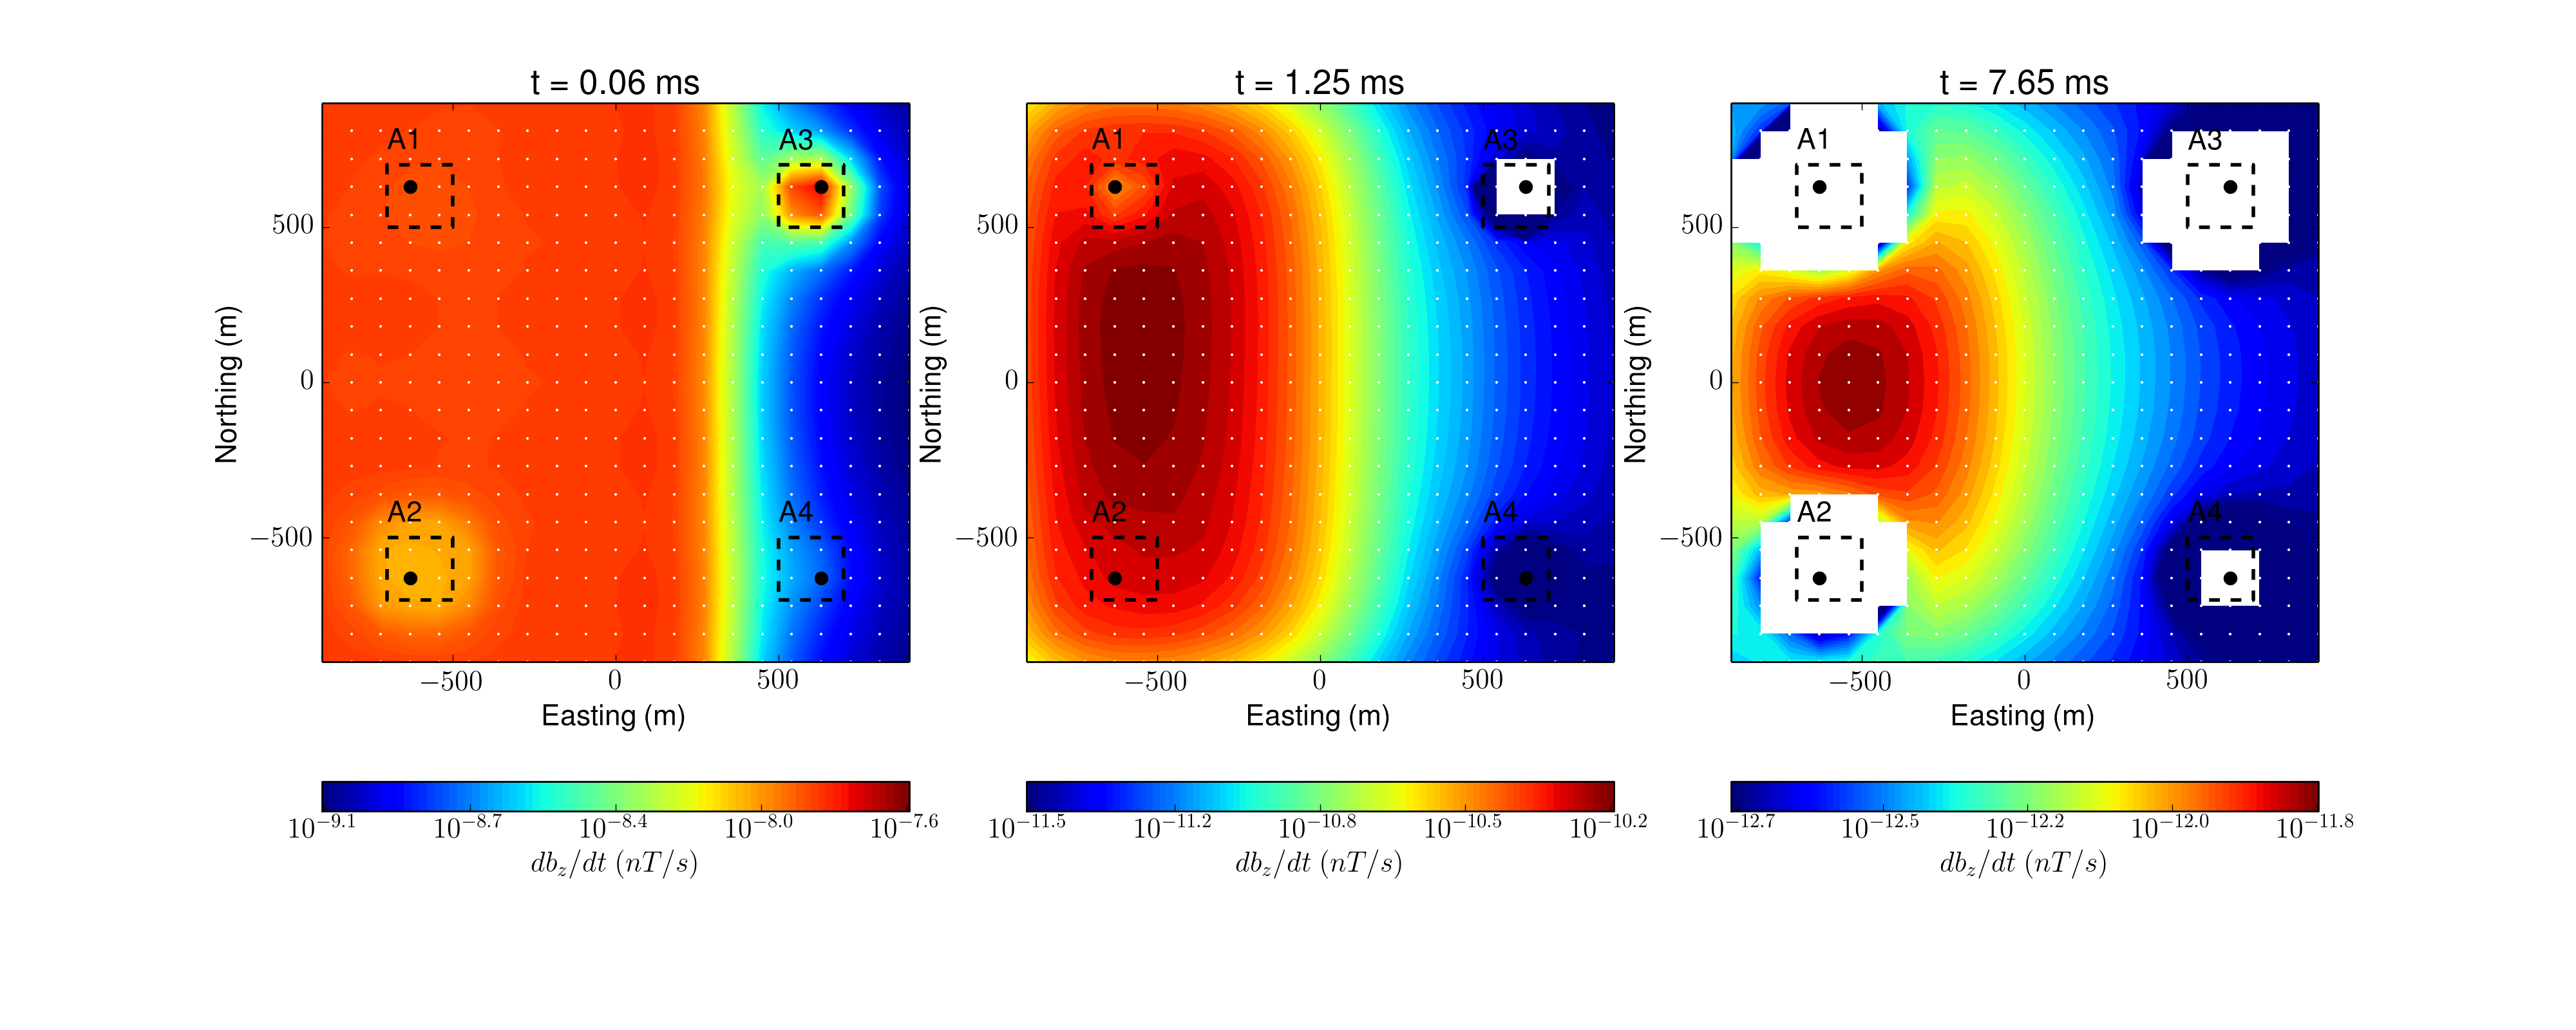
\includegraphics[width=1.0\textwidth]{figures/Totalmap.png}\\(a) Observed data ($d$)
  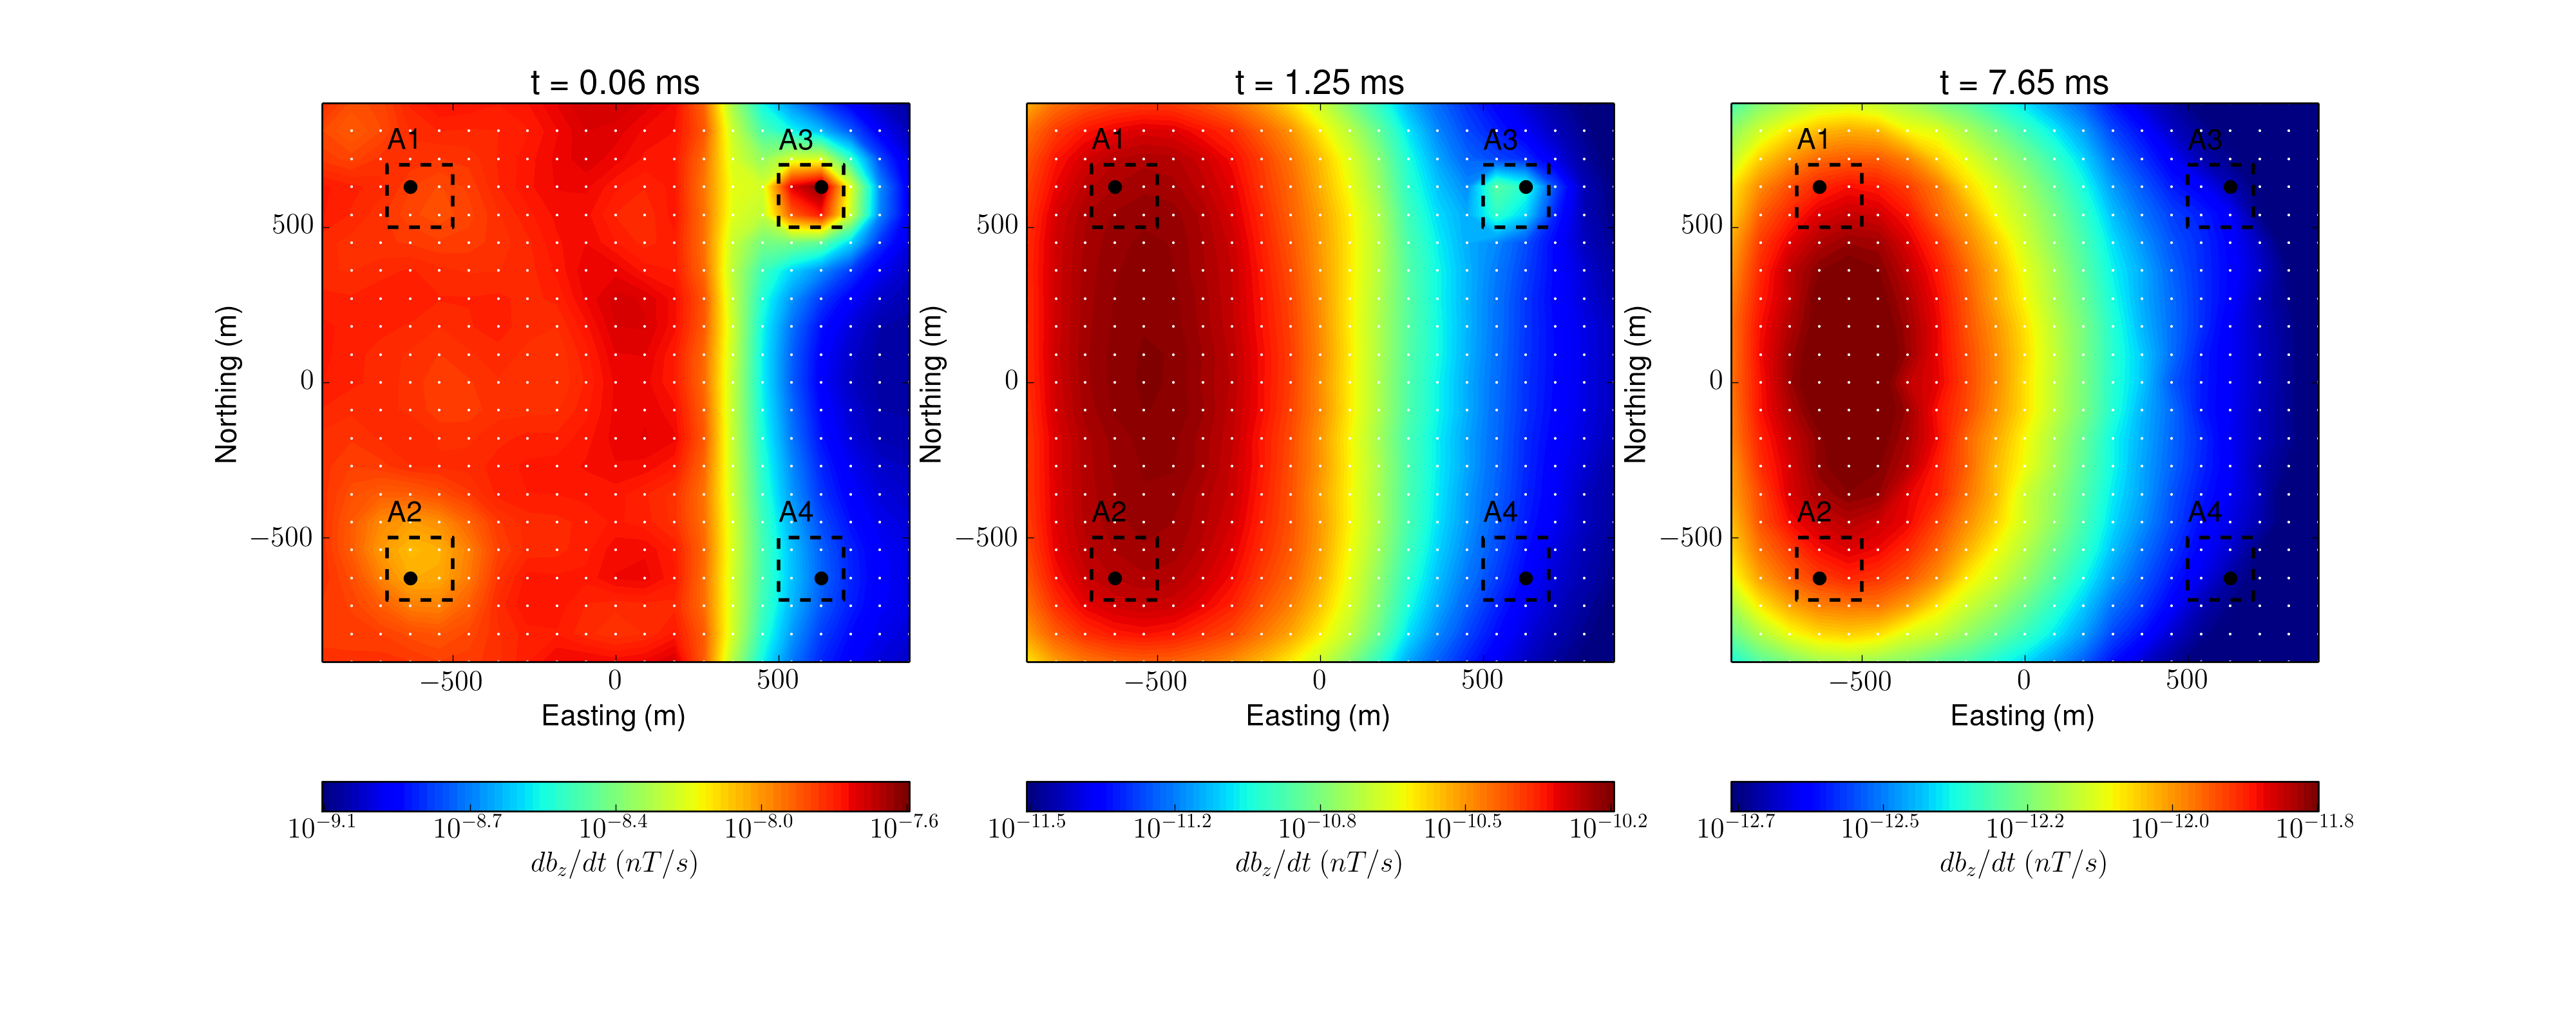
\includegraphics[width=1.0\textwidth]{figures/FundEstmap.png}\\(b) Predicted data ($d[\sigma_{est}]$)
  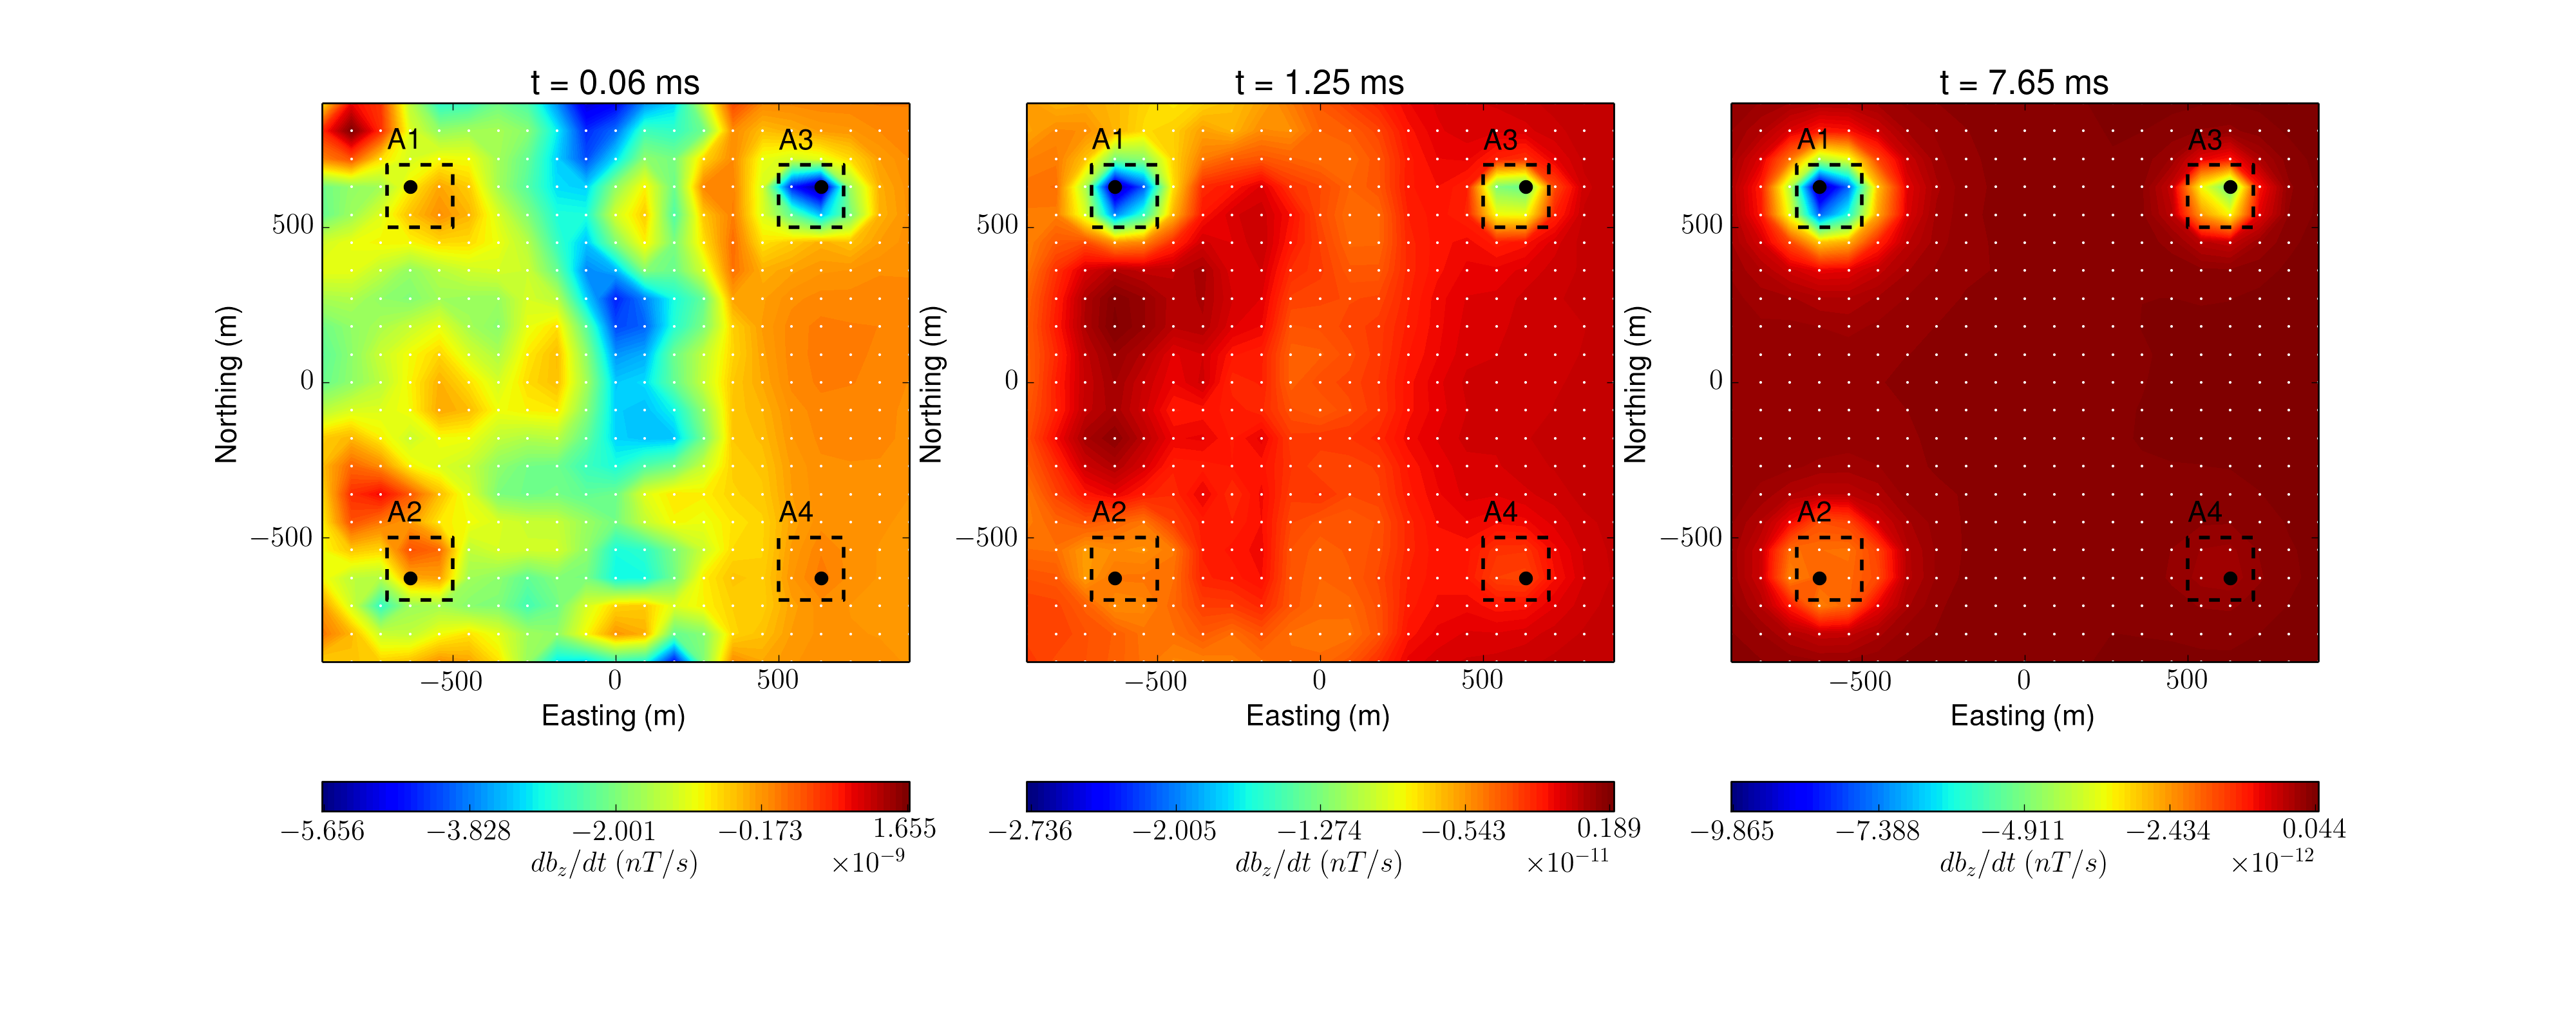
\includegraphics[width=1.0\textwidth]{figures/IPobsmap.png}\\(c) Raw IP data ($\dip_{raw}$)
  \caption{Observed ($d$), predicted ($d[\sigma_{est}]$, and raw IP ($\dip_{raw}$) responses. Left, middle and right panels correspondingly show times at 0.06, 1.25, and 7.65 ms). Dahsed lines contour horizontal boundary of four IP blocks (A1-A4).}
  \label{Fig:ObsPredIPResp}
\end{figure}

\begin{figure}[htb]
  \centering
  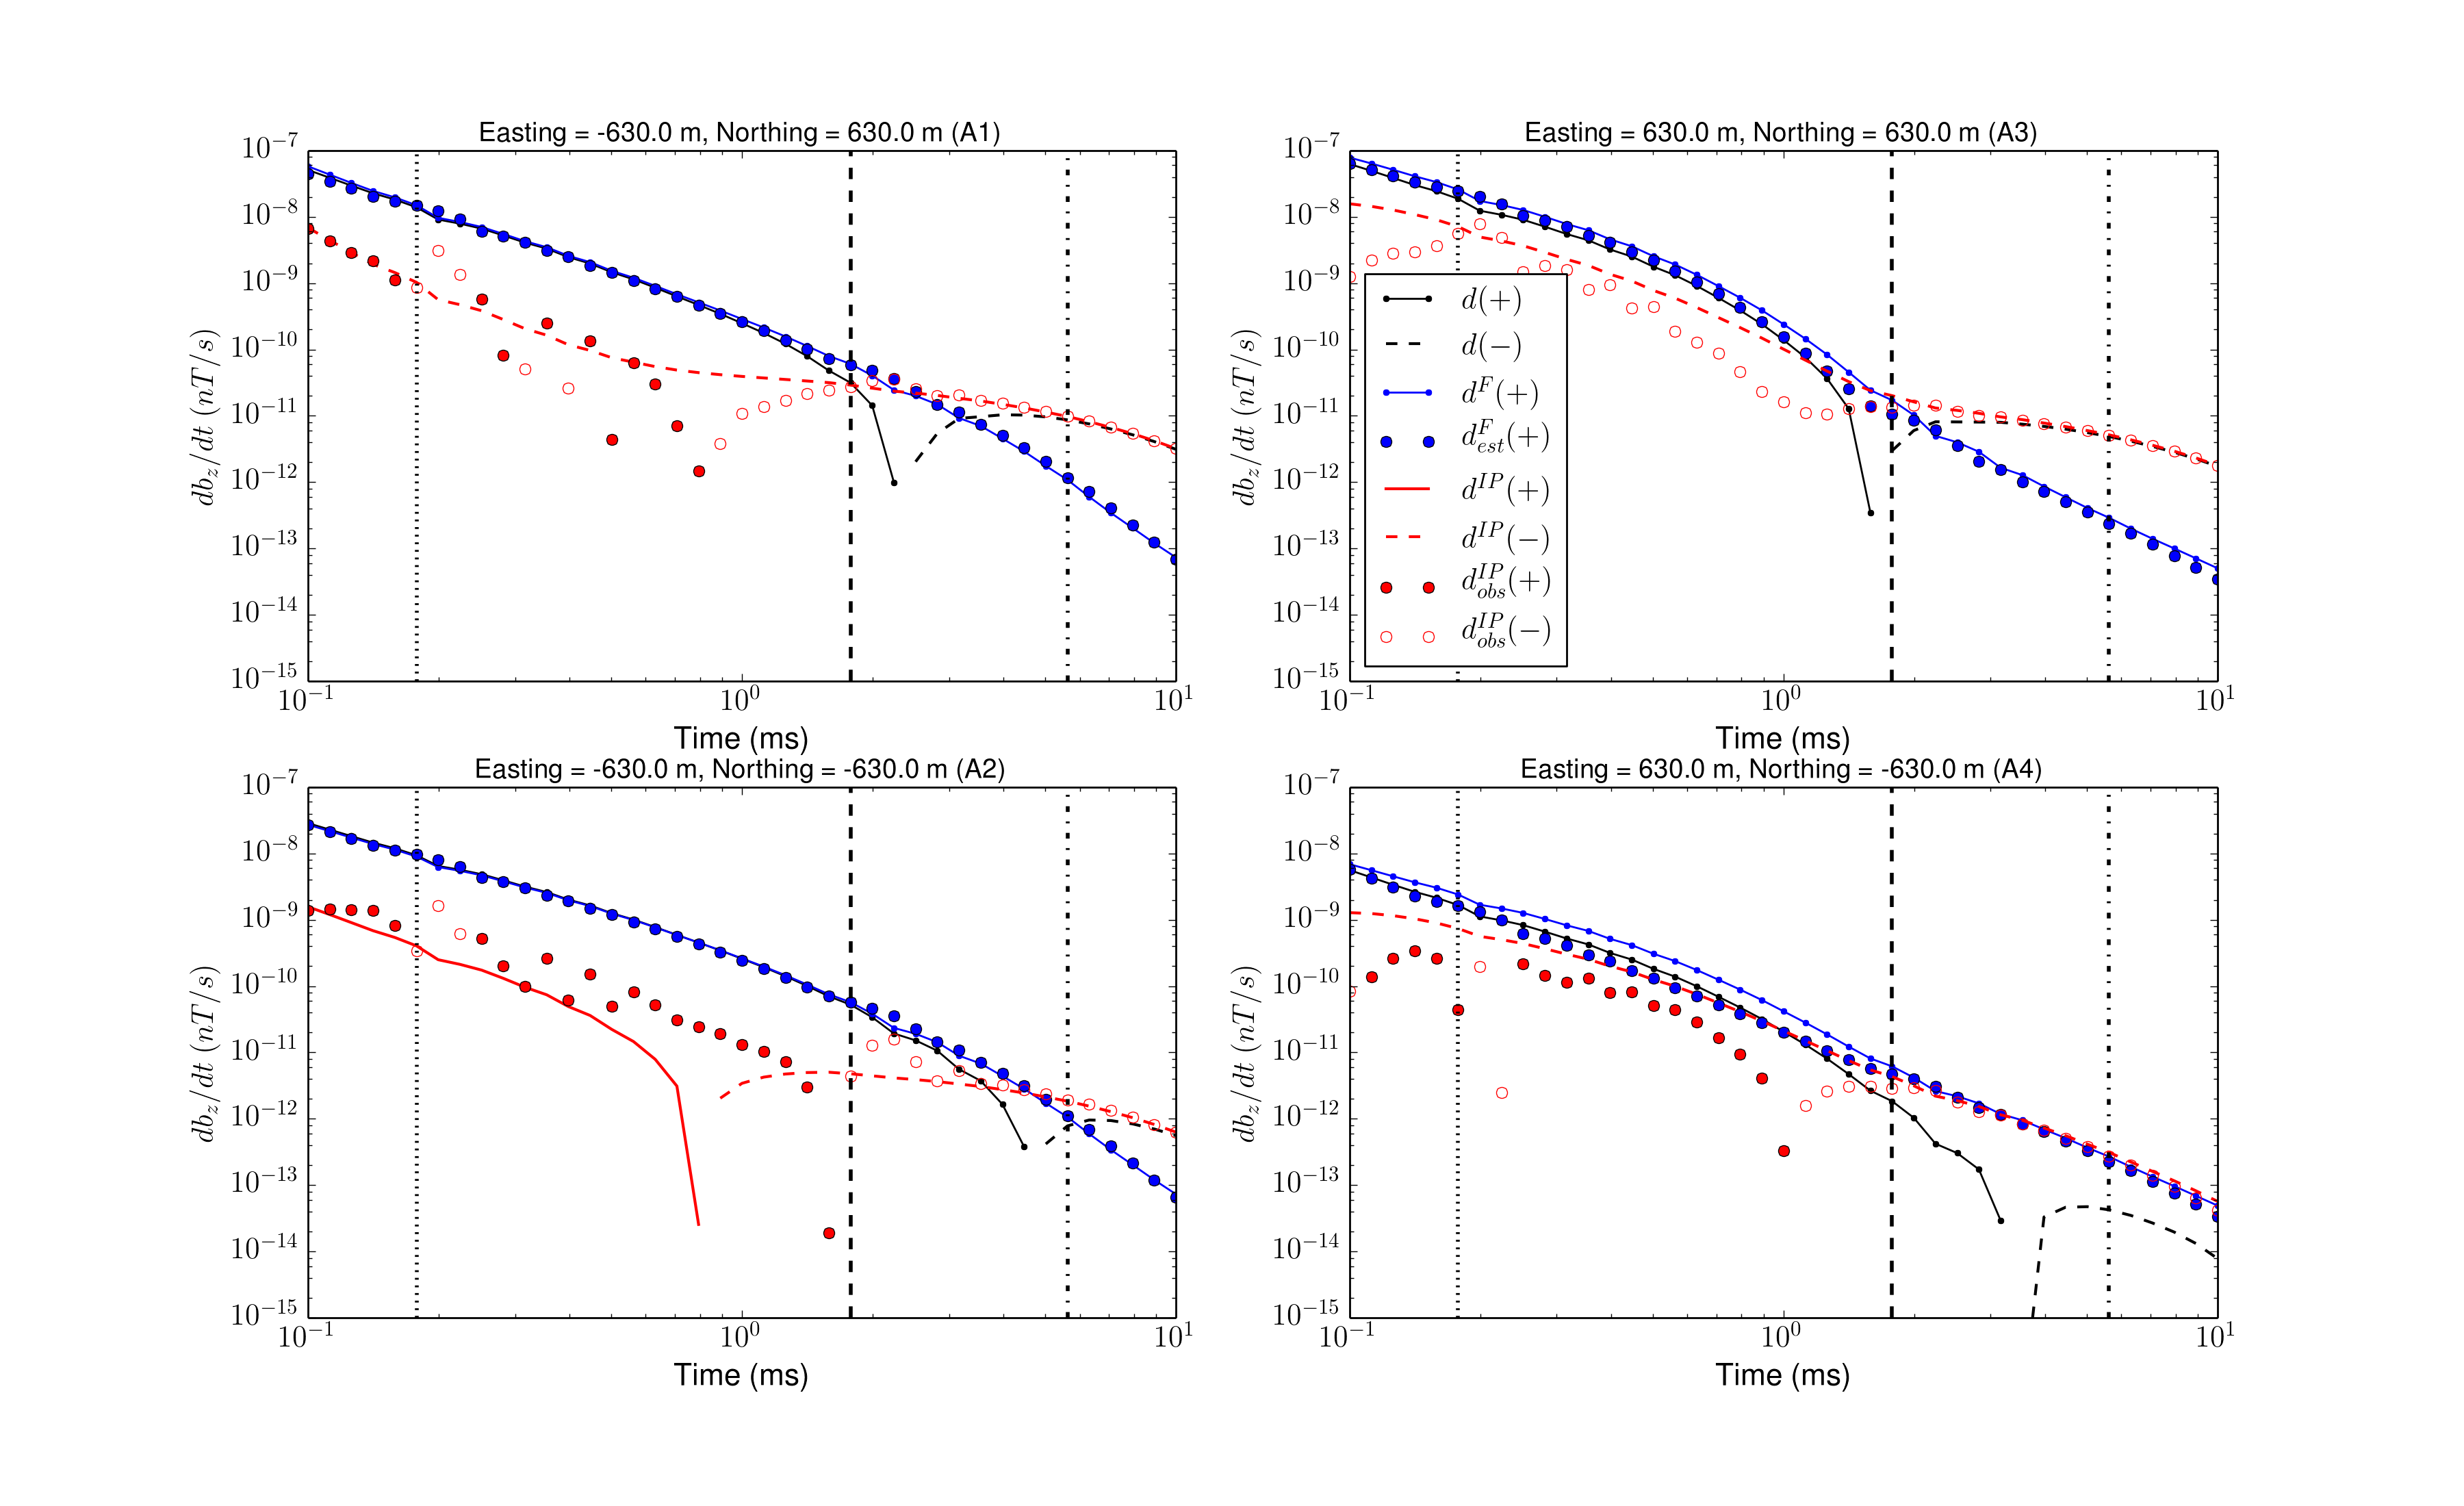
\includegraphics[width=1.0\textwidth]{figures/EMcurves.png}
  \caption{Transients of total (black lines), fundamental (blue lines), $\dip$ (red lines) and $\dip_{obs}$ (red circles) responses at four stations (A1-A4). Solid and dotted lines indicates positive and negative transients, respectively. Solid and empty lines indicates positive and negative transients, respectively.}
  \label{Fig:transientsall}
\end{figure}
\clearpage
\subsubsection{Regional removal}
As we commented briefly in the previous section, $\dip_{raw}$ will include some regional field  ($\triangle d[\siginf](t)$) due to the incorrect 3D conductivity model esitmated from 3D TEM inversion. To remove those regional field, we illustrate subtracion process corresponds to `regional removal' as
\begin{equation}
  \dip_{obs} = \dip_{raw}-\triangle d_{est},
\end{equation}
where $\triangle d_{est}$ is the estimated regional field. This procedure may important at `Effective' time range. However, at `No need' time range, this is not quite necessary similar to EM decoupling. We choose $\dip_{raw}$ at 1.25 ms (Effective) and apply a possible regional removal. 
On $\dip_{obs}$ map at 1.25 ms (middle panel of Fig. \ref{Fig:ObsPredIPResp}(c)), we can identify regional fields away from IP bodies. Assuming that we identified four anomalous $\dip$ responses, we fit $\dip_{obs}$ data as 6$^{th}$ order polynomial with exception of datum close to anomalies. White solid circles on $\dip_{obs}$ map (left panel of Fig. \ref{Fig:regremove}) indicate used stations to estimate regional fields. Estimated regional fields ($\triangle d_{est}$) are shown in the middle panel of Fig. \ref{Fig:regremove}. Then we subtract this estimated regional field from $\dip_{obs}$ and obtain corrected $\dip$ as shown in the right panel of Fig. \ref{Fig:regremove}. We reduced regional fields reasonably. We can recognize that a proper regional removal step possibly be needed in practice. However, the importance of this processing decreases as we go later time channels.

Further researches are needed to make EM decoupling and regional removal processes more robust, because current approach is considerably dependent on how well we perform 3D TEM inversion. 

\begin{figure}[htb]
  \centering
  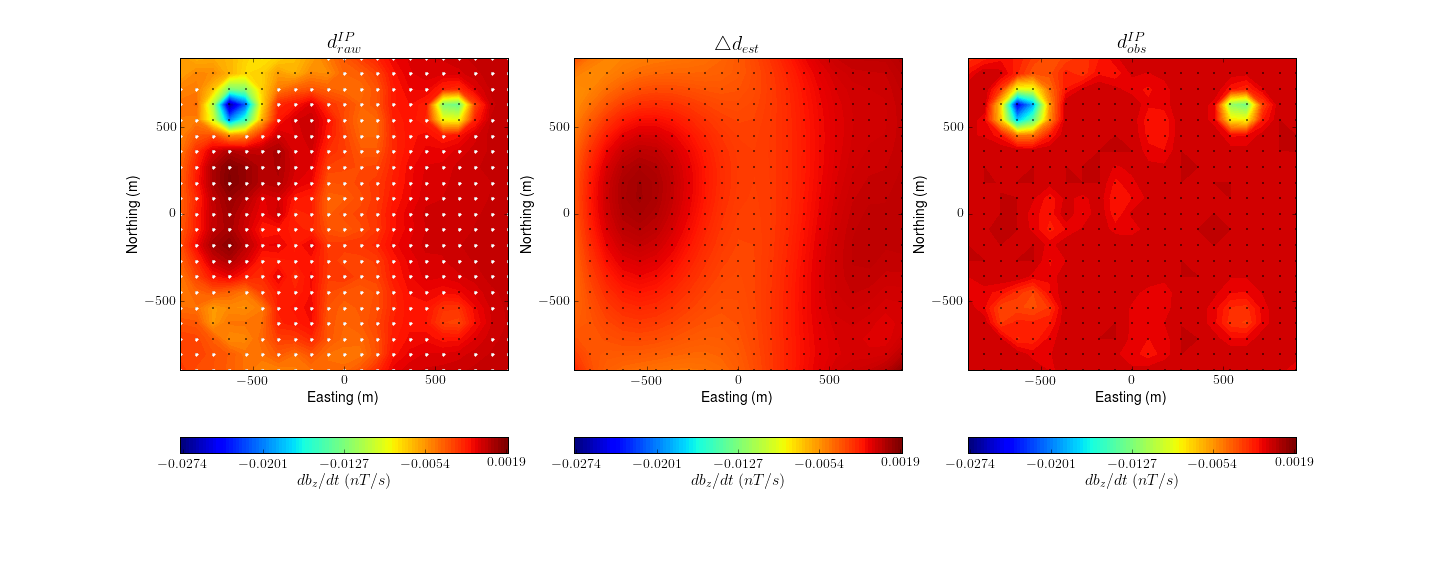
\includegraphics[width=1.0\textwidth]{figures/RegRem_field_1_25ms.png}
  \caption{Regional removal procedure. Left, middle and right panels correspondinlgy indicate $\dip_{raw}$, $\triangle d_{est}$ and corrected $\dip_{obs}$. Black dots and solid white circles indicate locations of stations and stations used to estimate regional field.}
  \label{Fig:regremove}
\end{figure}

\subsubsection{IP inversion}
Using the EM decoupling method in the previous section, we recognized $\dip$ responses embedded in the observed ATEM data. Natural next step is an IP inversion to recover 3D distribution of pseudo-chareability. We apply 3D IP inversion to $\dip_{obs}$ responses at 1.25 ms shown in the right panel of Figure ~\ref{Fig:regremove}. The inversion model in this example is $(\petadt)_i$ where subscript $i$ indicates $i^{th}$ time channel. Depending on the types of data, either $\b$ or $\dbdt$, the inversion recover either $(\peta)_i$ or $(\petadt)_i$. For convience of the notation for following inversion analyses, we call $(\petadt)_i$ as pseudo-chargeability as well. Note that we only use $\dbdt$ data in this study, any inverted model we will show is $(\petadt)_i$.
Fig. \ref{Fig:petaestmodel_syn} show recovered pseudo-chareability model. Four chargeable bodies are recovered. 

\begin{figure}[htb]
  \centering
  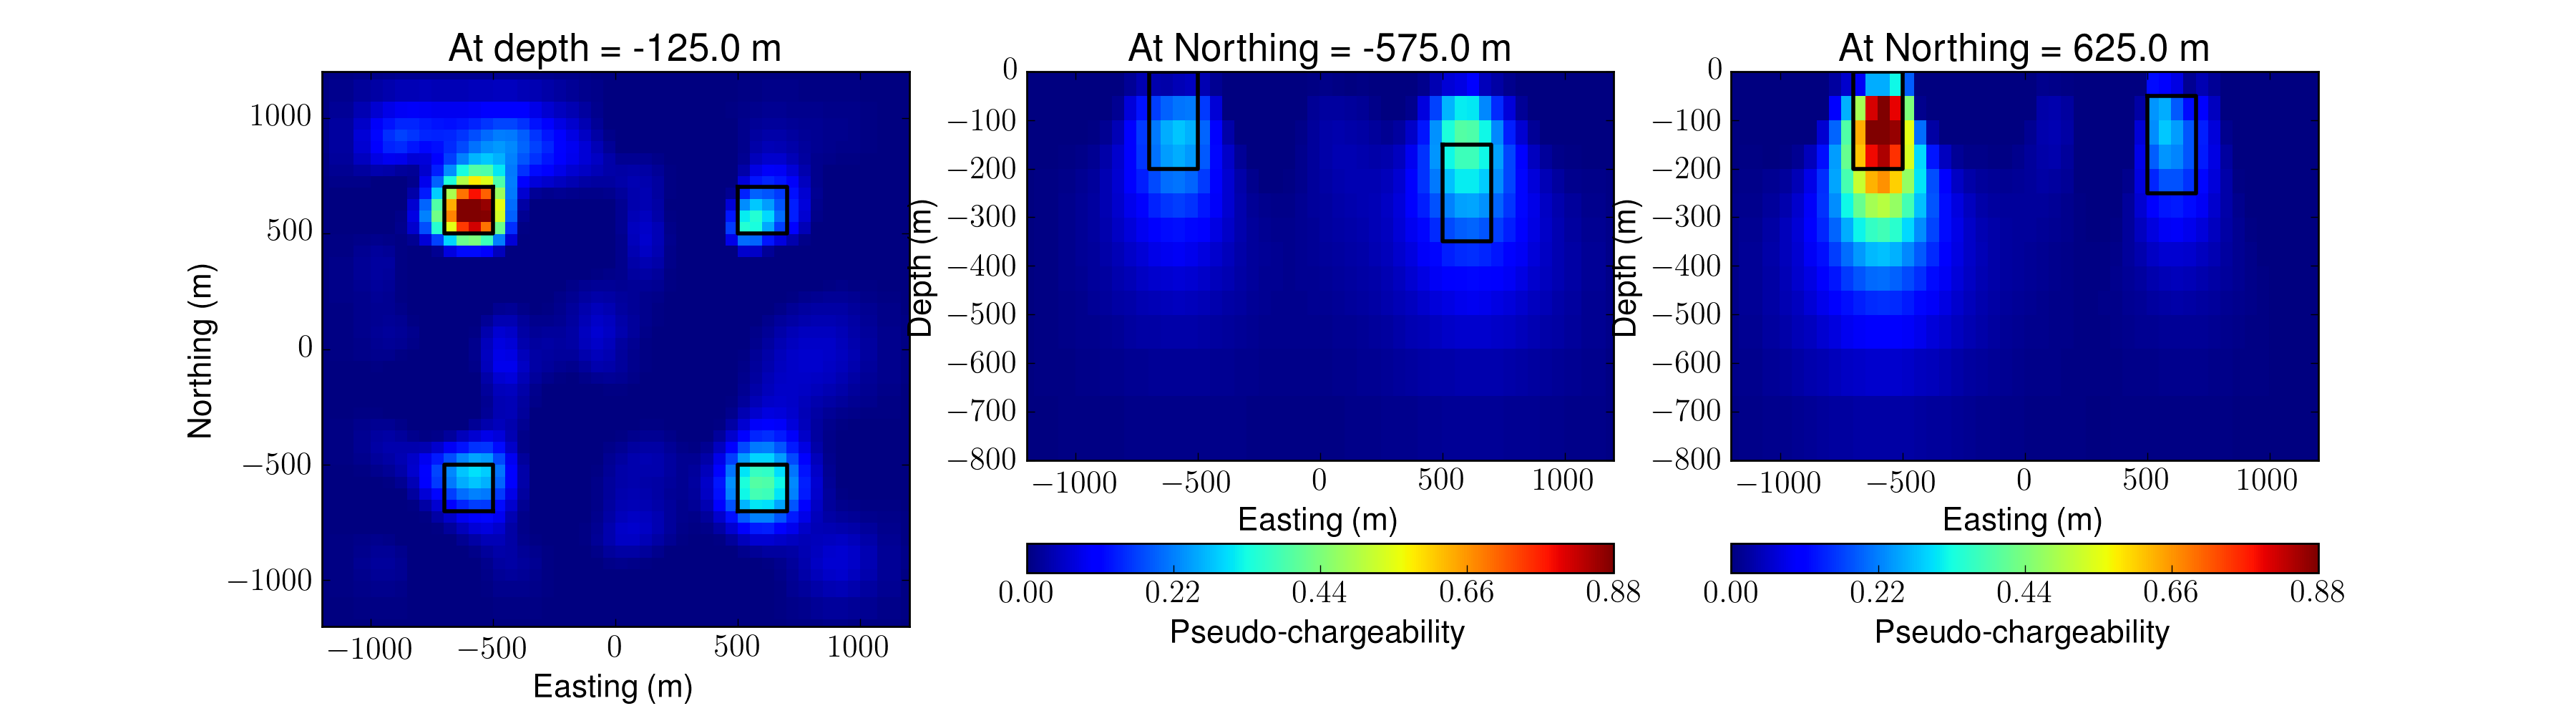
\includegraphics[width=1.0\textwidth]{figures/Petaest_reg_1_25ms.png}
  \caption{Sectional view of the recovered pseudo-chargeability model at 1.25 ms.}
  \label{Fig:petaestmodel_syn}
\end{figure}

\subsection{Field example: Mt. Milligan}
We apply ATEM-IP inversion workflow to the Mt Millgian VTEM data. Three time channels of the observed response are shown in Fig. ~\ref{Fig:response_field}(a). The observed data at 7.1 ms, which is the latest time channel that was used in the ATEM inversion, cleary shows two distingtive negative anomalies (A2 and A3). Here blanked region indicates negative values. However, in earlier times (4.6 and 5.1 ms), responses are postive on these locations. Using the 3D conductivity from \cite{yang20143}, we computed predicted response (Fig. ~\ref{Fig:response_field}(b)). Subtraction of this predicted response from the observation yields $\dip_{raw}$ (Fig. \ref{Fig:response_field}(c)). On computed $\dip_{raw}$ maps at 7.1 ms, we first identify IP anomalies near A2 and A3, where we observed negative values in the observed data and these are marked as black dahsed circles. In addition, we identify three more IP anomalies (A1, A4 and A5), which we could not observe any negative response, and they are marked as white dashed circles. We can observe similar features in $\dip$ map at 5.1 ms. Performance of the EM decoupling process decreases as we go earlier time (4.6 ms). 

The next stp is to account for inexact knowledge about the background conductivity. For each time channel we estimate regional by fitting the observed data with a 5th order polynomial then subtract this regional($\triangle d[\siginf]$) from $\dip_{raw}$. The $\dip_{obs}$, the estimated regional and the corrected $\dip$ data at 7.1 ms are shown in Fig. ~\ref{Fig:regremoval_field}. These maps convey much information of existence of IP anomalies. 

The final step is to carry out the IP inversion. In Fig. ~\ref{Fig:Peta_field}(a), we present a 3D pseudo-chargeability model, which is recovered from the 3D IP inversion of $\dip$ data at 7.2 ms.  We can identify anomalous $\dip$ responses are reasonably mapped in the 3D space, and we also observe the changes of anomalous IP bodies in depth. 

\begin{figure}[htb]
  \centering
  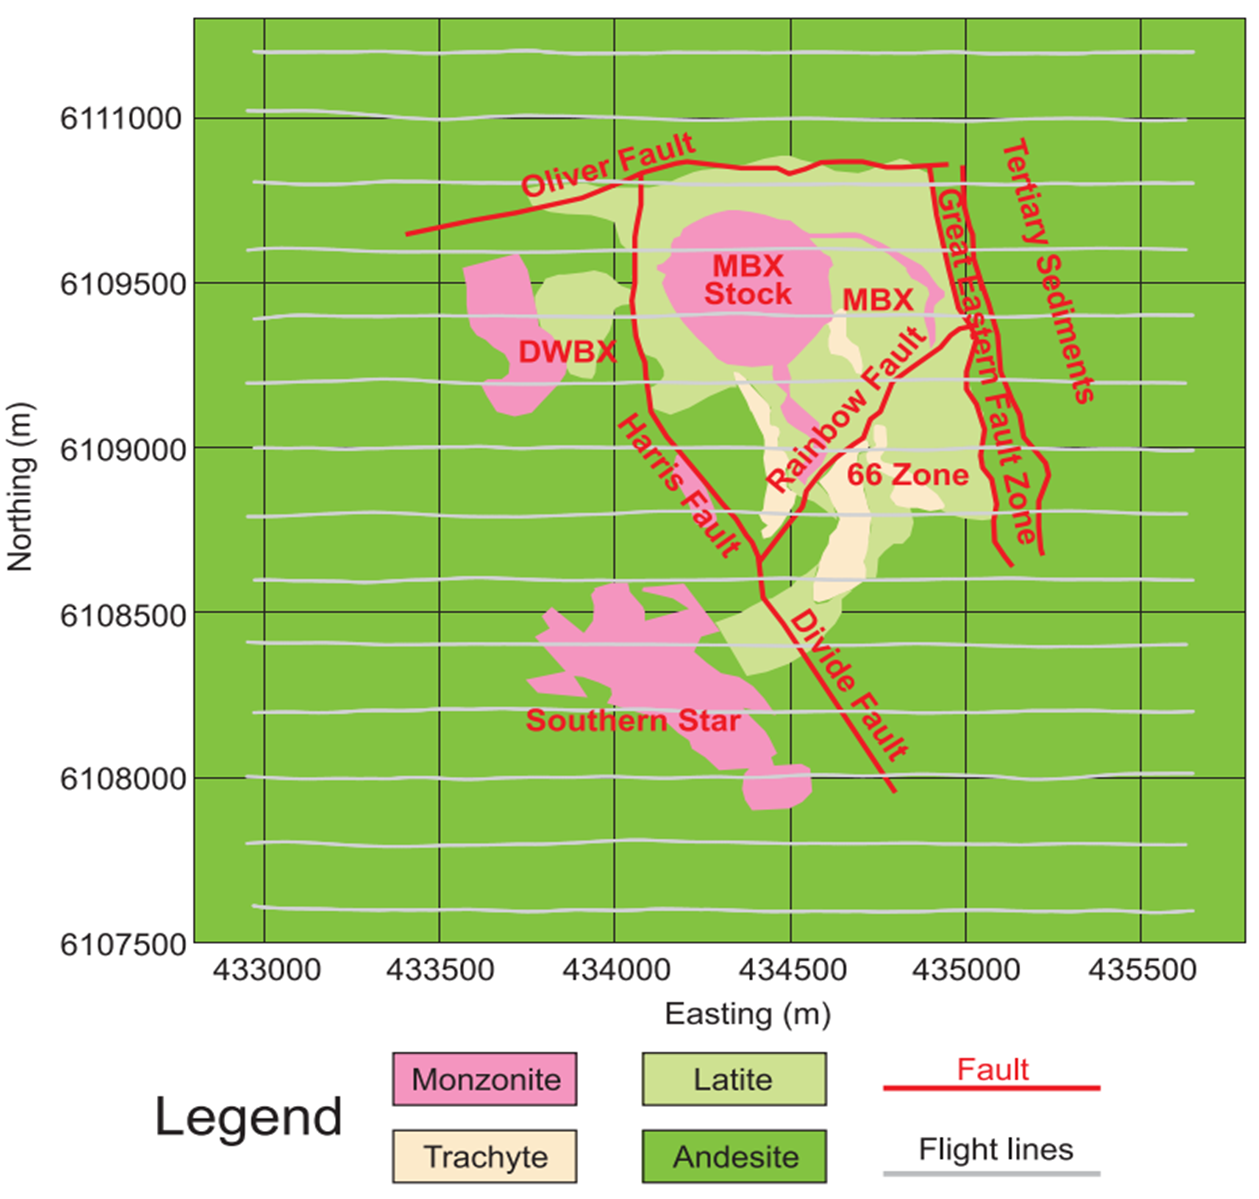
\includegraphics[width=0.6\textwidth]{figures/milligan_geo.png}
  \caption{Geology and VTEM survey at Mt Milligan porphyry deposit in British Columbia, Canada. (\cite{yang20143}).}
  \label{Fig:milligan_geology}
\end{figure}

\begin{figure}[htb]
  \centering
  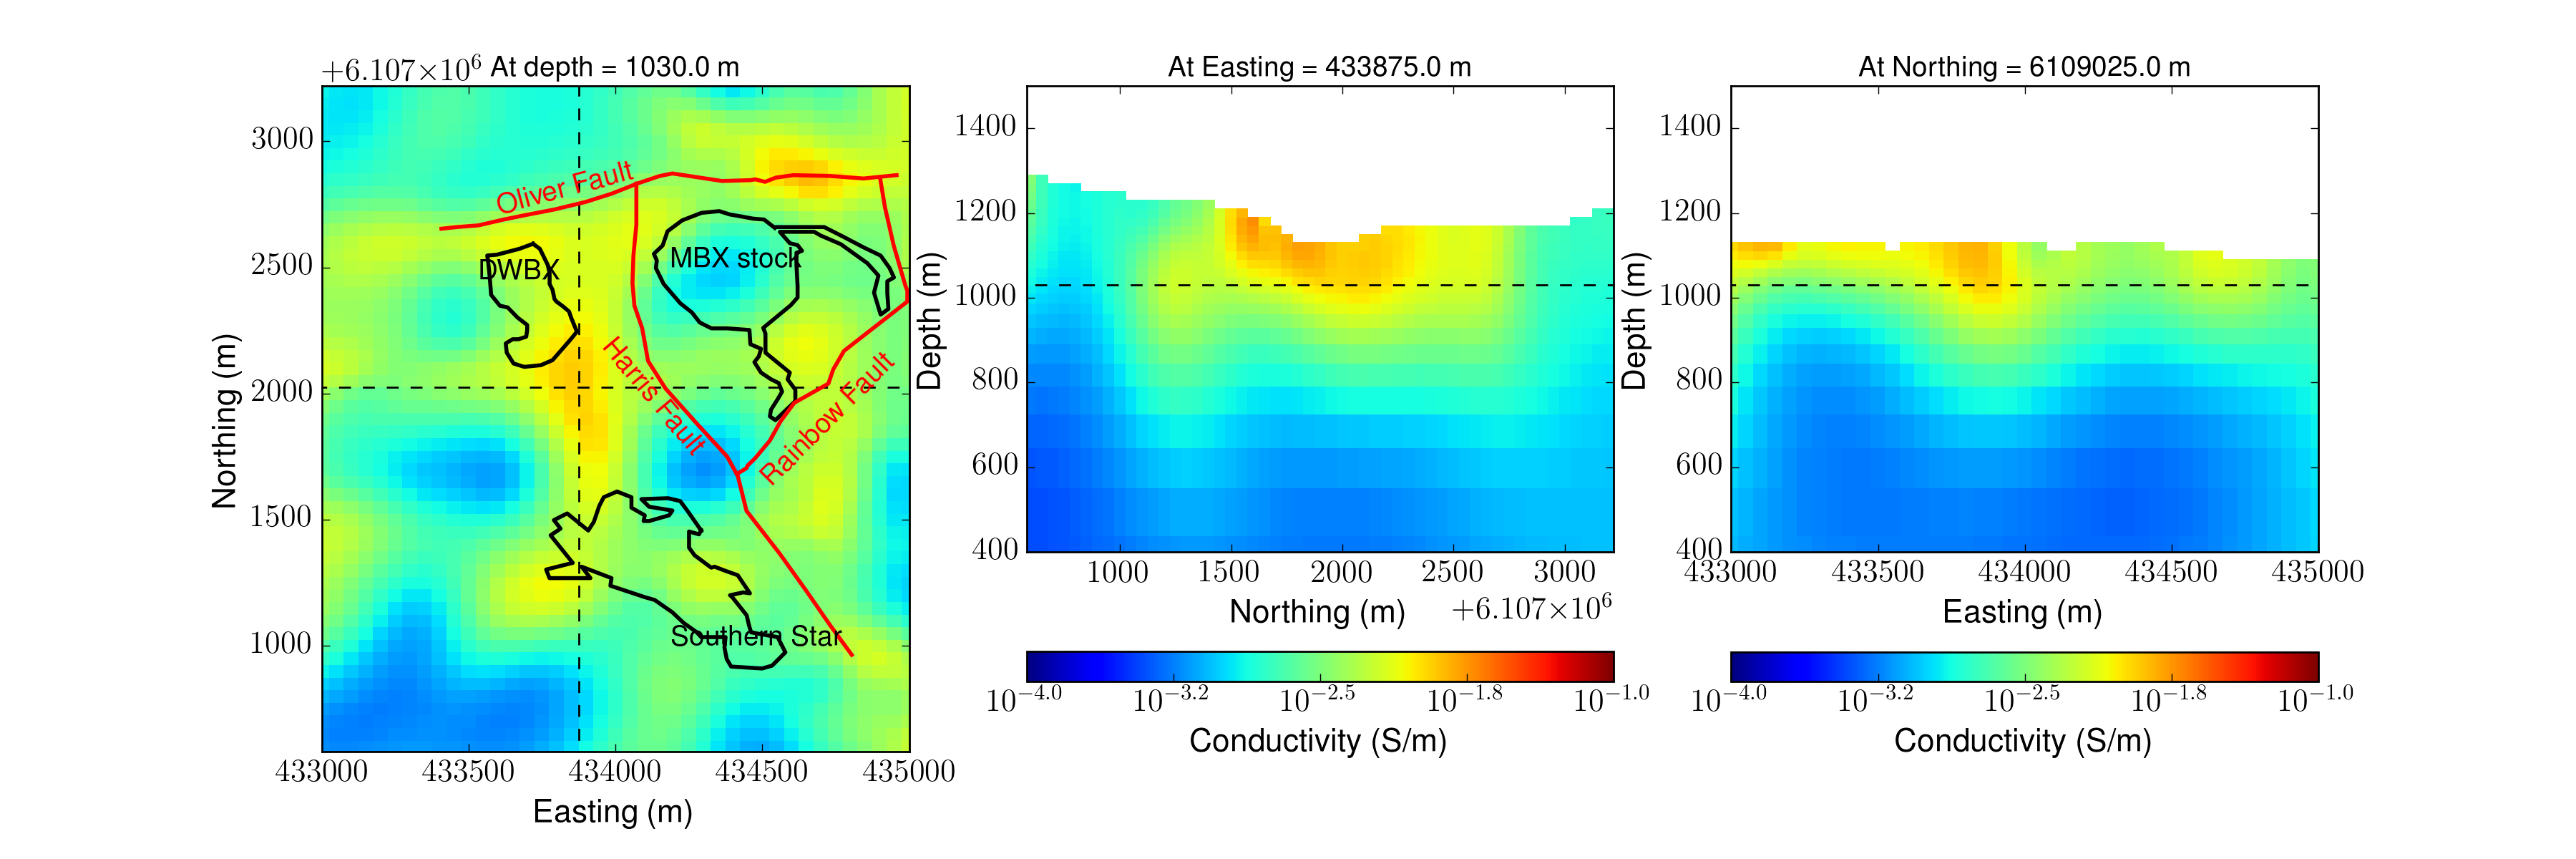
\includegraphics[width=1.0\textwidth]{figures/sigma_est_field.png}
  \caption{3D Conductivity model of Mt Milligan example. 3D ATEM inversion has been peformed by \cite{yang20143}.}
  \label{Fig:milligan_sigma}
\end{figure}

\begin{figure}[htb]
  \centering
  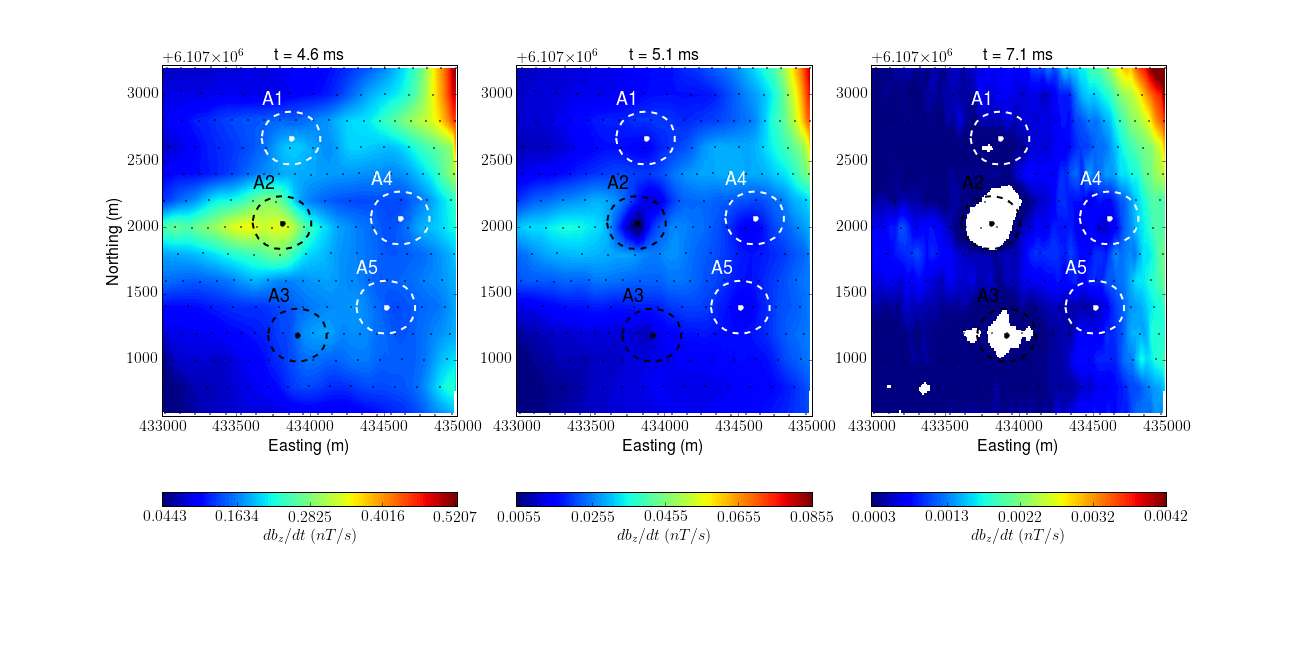
\includegraphics[width=0.7\textwidth]{figures/OBS_field.png}\\ (a) Observed data ($d$) \\
  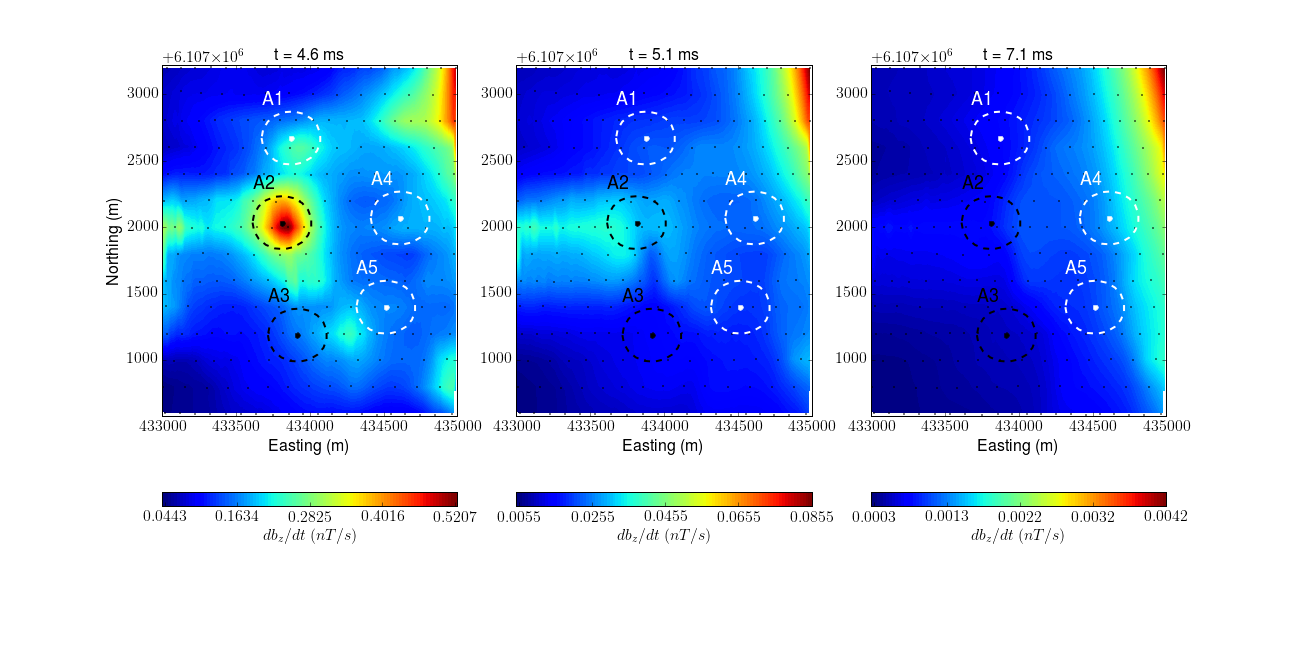
\includegraphics[width=0.7\textwidth]{figures/FUND_field.png}\\ (b) Predicted data ($d[\sigma_{est}]$)\\
  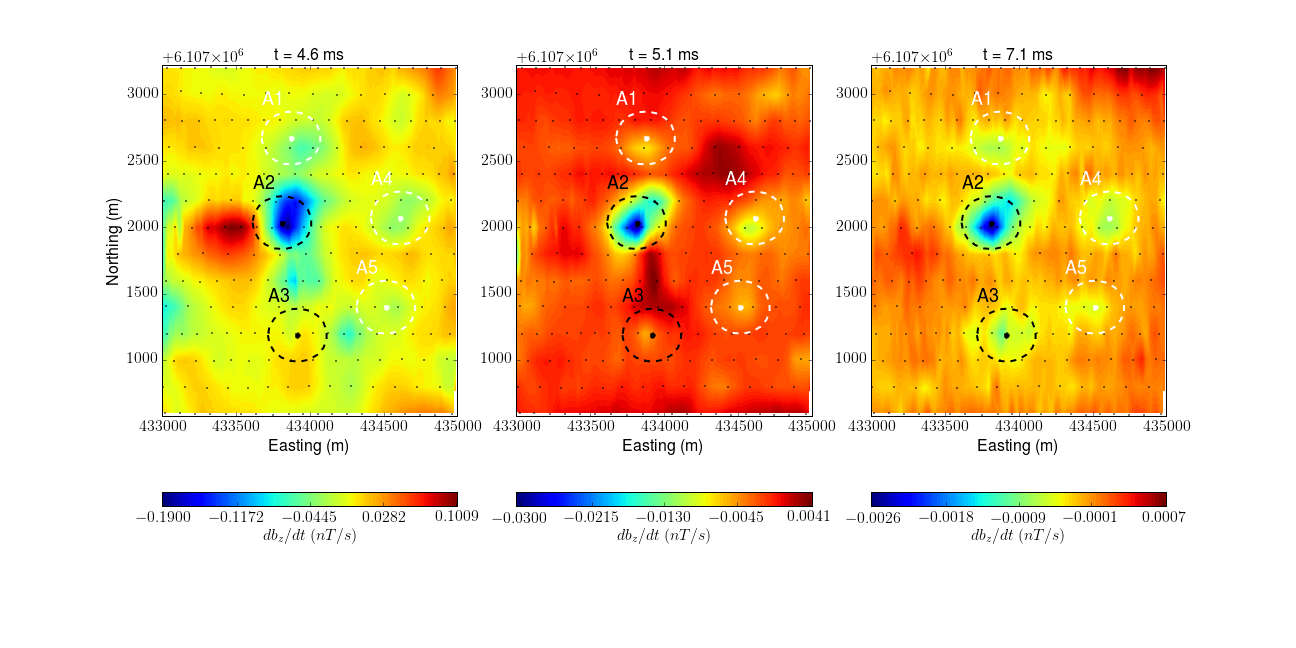
\includegraphics[width=0.7\textwidth]{figures/dIP_field.png} \\ (c) Raw IP data ($\dip_{raw}$)
  \caption{Comparisons of the observed, predicted and $\dip_{raw}$ data Mt Millgian region. (a) Observed, (b) predicted, and (c) $\dip_{obs}$ data. Right, middle and left panel indicate times at 4.8, 5.1, and 6.4 ms. Black dashed circles (A2 and A3) indicate IP nomalies where we can observe negatvie response. White dashed circles (A1, A4 and A5) indicate those we cannot observe negative.}
  \label{Fig:response_field}
\end{figure}

\begin{figure}[htb]
  \centering
  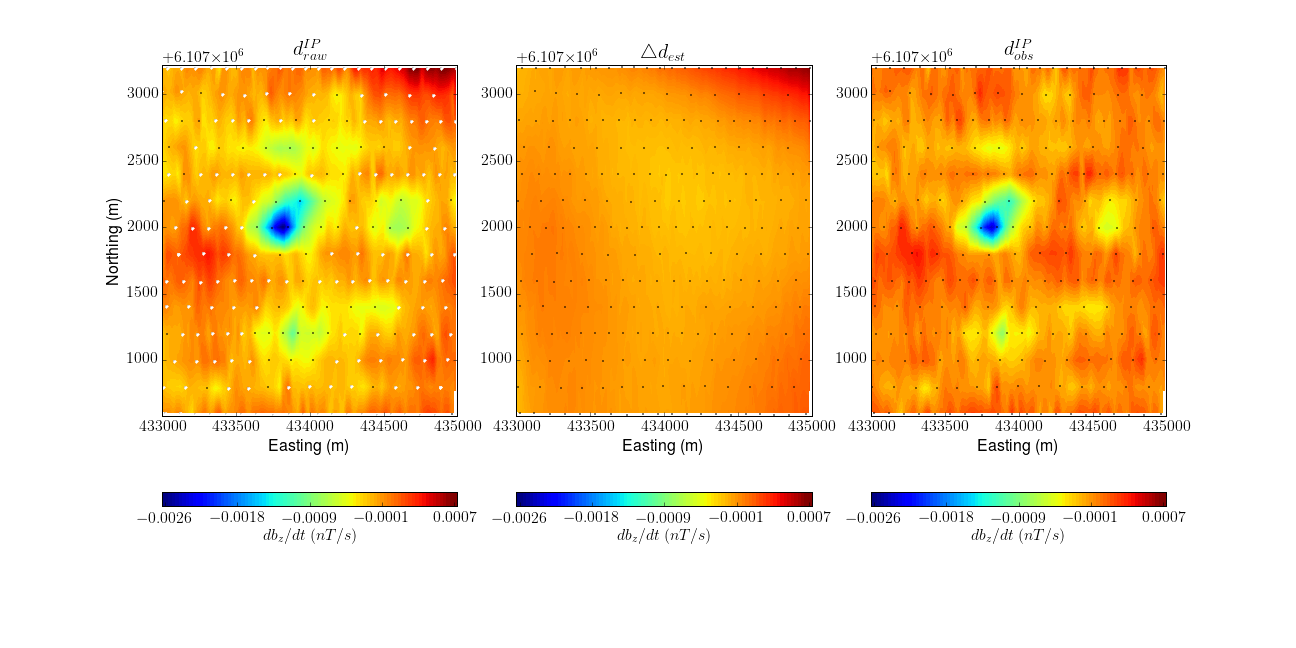
\includegraphics[width=0.8\textwidth]{figures/RegRem_field_ch7.png}
  \caption{Regional removal of Mt Milligan ATEM data. Left, middle and right panels correspondinlgy indicate $\dip_{raw}$, $\triangle d_{est}$ and $\dip_{obs}$. Black dots and solid white circles indicate locations of stations and stations used to estimate regional field.}
  \label{Fig:regremoval_field}
\end{figure}

\begin{figure}[htb]
  \centering
  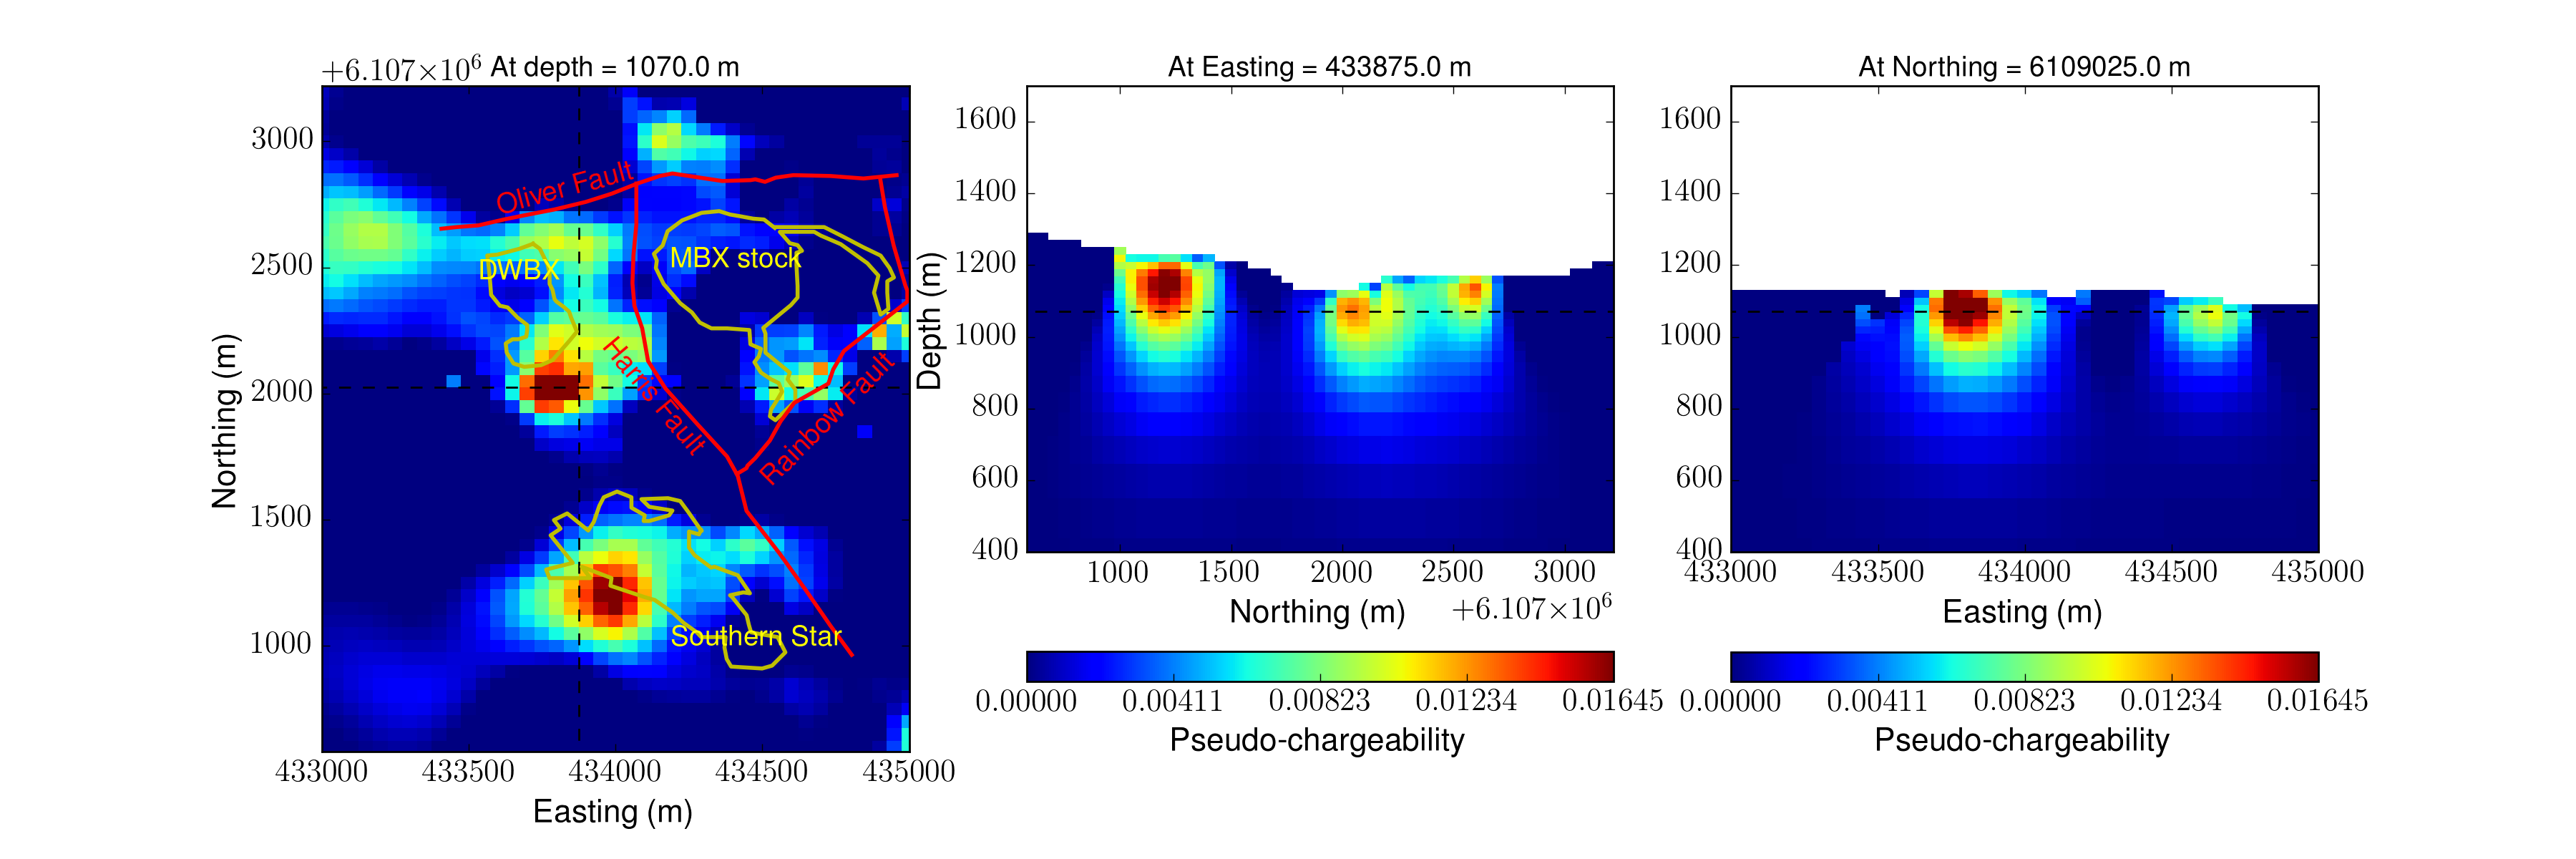
\includegraphics[width=1.0\textwidth]{figures/Peta_field.png}
  \caption{Section views of the recovered 3D pseudo-chargeability model.}
  \label{Fig:Peta_field}
\end{figure}
\clearpage

\section{CONCLUSIONS}
We have developed an IP inversion workflow to recover 3D distribution of IP information from TEM data. The processing contains estimation of a background conductivity, removal of EM coupling, estimation of a possible residual field induced by incorrect conductivity distribution of the earth, and carrying out a 3D inversion to recover a pseudo-chargeability. To realize this workflow, mathematical foundations were constructed by decomposition of the observed EM fields and the linearization of IP responses as a function of pseudo-chargeability. Different excitation mechanism of inductive source from galvanic source was carefully considered to construct a linear form of IP response. 

For the remainder of my Ph.D., the primary areas of research will be:
\begin{itemize}
  \item Applying our IP inversion procedure for galvanic source IP surveys (EIP and MIP)
  \item Extracting intrinsic IP information such as Cole-Cole parameters
  \item Connecting recovered IP information to possible geological sources of IP
  \item Depth resolution of airborne IP
\end{itemize}

\subsection{Intellectual merits and impact}
In contrast to galvanic source IP, which is a matured technique in mining application, exploiting IP effects in inductive source system is still young technique. Most of interpretations about ISIP is based on one-dimenional approach. We treated ISIP problem in 3D, and constructed linear functional which simulates ISIP responses, and tested. There are two important aspects that this linear functional provides:
\begin{itemize}
  \item Physical understanding of polarizatoin charge build-up and its impact to the observed data
  \item Cost effective forward modelling which allows us to run fast 3D IP inversion
\end{itemize}
In addition,  we suggested a comprehensive IP inversion procedure, which can be applied to both galvanic and inductive sources TEM data. We are planning to apply this procedure to different types of IP data including EIP, MIP, and ISIP. This will provide a comprehensive methodolgy that one can obtain 3D distribution of IP information from TEM data.

\subsection{Research timeline}
\begin{enumerate}
  \item Linearization of time domain IP data and applying the IP inversion procedure
  \begin{itemize}
    \item Inductive source (\cite{Kang2015c}, submitted to $\mathit Geophysical \ Journal \ International$)
    \item Galvanic source (on-going)
  \end{itemize}
  \item Airbonre IP
  \begin{itemize}
    \item EM decoupling and 3D IP inversion (\cite{Kang2015a}, preparing a paper to submit $\mathit Geophysics$)
    \item Airborne IP for Kimberlite explorations (\cite{Kang2015b}, preparing a paper to submit $\mathit Geophysics \ Interpretation$)
    \item Depth resolution of airborne IP
  \end{itemize}  
\end{enumerate}
\subsection{Relevant conference presentations - (* = presenting author)}
\begin{itemize}
\item
$\mathbf{Kang, S.}$*, Oldenburg, D. W., (2014), On recovering induced polarization information from airborne time domain EM data, $SEG \ Extended \ Abstracts$ - Winner: Best student talk, Mining Section.
\item
$\mathbf{Kang, S.}$*, Oldenburg, D. W., (2015), Recovering IP information in airborne-time domain electromagnetic data, $ASEG \ Extended \ Abstracts$.
\item
$\mathbf{Kang, S.}$*, Oldenburg, D. W., (2015), 3D IP Inversion of Airborne EM data at Tli Kwi Cho, $ASEG \ Extended \ Abstracts$.
\item
$\mathbf{Kang, S.}$*, Rowan, C., Lindsey, H., and Oldenburg, D. W., (2015), Moving between dimensions in EM inversions, $SEG \ Extended \ Abstracts$.
\end{itemize}

\subsection{Peer reviewed publications}
\begin{itemize}
\item
Rowan, C., \&, $\mathbf{Kang, S.}$, \& Lindsey, H., Pidlisecky, A., and Oldenburg, D. W., (2015). SimPEG: An Open Source Framework for Simulation and Gradient Based Parameter Estimation in Geophysical Applications, $\mathit Computers \ and \ Geoscience$.
\item 
$\mathbf{Kang, S.}$, \& Oldenburg, D. W., (2015). On recovering distributed IP information from inductive source time domain electromagnetic data,  $\mathit Geophysical \ Journal \ International$ (submitted).
\end{itemize}
%%%%%%%%%%%%%%%%%%%%%%%%%%%%%%%%%%%%%%%%%%%%%%%%%%%%%%%%%%%%%%%%%%%%%%%%%%%%%%%
\newpage
\bibliographystyle{plain}
% \bibliographystyle{C:/SEGTex/SEG2014/seg}
\bibliography{reference}


\end{document}

